\chapter{Introduction\label{ch:intro}}

Since the advent of the information age with the completion of the
first transistor-based computer in 1954, Moore's law has ensured a
steady decrease in the cost of computation. The concomitant rise in
simulation complexity paired with the proliferation of electronic
sensors has resulted in a torrent of data; the CERN Data Centre alone
proccesses around one thousand terabytes daily. To address the
challenge of separating the valuable bits from the uninformative, a
host of machine learning techniques have been developed, ranging from
the simplistic but venerable principal component analysis to complex
neural networks. Their successes are numerous. Principal component
analysis has been used to analyze PET scans \cite{friston_functional_1993}, to predict traffice flow \cite{zhang_forecasting_2007}, and to examine groundwater composition
\cite{helena_temporal_2000}. Neural networks can automatically segment images and
classify videos \cite{karpathy_large-scale_2014,zheng_conditional_2015}, and logistic regression has been used to
detect gene interactions \cite{park_penalized_2008}. These are but a few of the thousands
of successful applications of machine learning algorithms to large
datasets.

Despite this progress, the problem demands continuous innovation to
match the growing variety and supply of data. Dimensionality
reduction, the problem of describing a set of data in the fewest
number of variables possible without discarding important information,
is an increasingly imporant area of investigation. Dimensionality
reduction can reveal simpler ways of viewing a system, directing
researcher's attention to the few significant variables hidden in
their experimental output. Alternatively, it is often used as a
crucial pre-processing step when implementing machine learning models,
accelerating optimization. The work presented in this thesis focuses
on advances of the former type, where the algorithms we develop yield
insight into the important factors driving a system. In particular we
target the fields of complex networks and parameter estimation.

Defined as a set of items and the connections between them \cite{newman_structure_2003}, networks provide a
useful framework for modeling many real-world systems. In biology,
protein-protein interaction networks have been used to identify
distinct collections of proteins that are conserved across species
\cite{wuchty_evolutionary_2003}. Economist have constructed network
models of trade and determined that highly connected networks are more
sensititve to price variations \cite{li_spatial_2008}. Applications can even be found in
linguistics, where semantic network analysis indicates that
well-structured speeches win presidential debates \cite{Semantic
  networks and competition: Election year winners and losers in
  U.S. televised presidential debates, 1960–2004} (note that this
study included no data from 2016).

Regardless of the specific system, researchers often seek an
understanding of some emergent, macroscopic behavior. In
epidiemological models composed of thousands of interacting
individuals, often just the overall fraction that is infected is of
interest \cite{shi_sis_2008}. Ideally an analytical equation governing
the evolution of the quantity of interest would be readily derived
from a description of the fine-scale dynamics; however, as model
complexity increases in an effort to better match real-world
conditions, deriving such closed-form expressions becomes increasingly
difficult. In such cases, equation free modeling may enable the
desired macroscopic analysis despite the lack of explicit
equations. This approach has been successfuly applied to simple models
of network evolution \cite{bold_equation-free_2014}, and we extend
this work to hypergraph models in which multiple connections are
permitted between nodes.

Often the goal is even more basic: to determine whether a
low-dimensional description of the model exists in the first place. In
many models of network generation, the parameters that influence the
network structure are clear, see for instance
\cite{erdos_random_1959,chung_connected_2002,watts_collective_1998,
  Barabasi}. In more complicated models the picture is muddier, and it
would helpful to have an automated method of identifying whether such
a simpler description is present. Towards this end, we extend the
dimensionality-reduction technique Diffusion Maps to parameterize
collections of hypergraphs. This requires a suitable measure of the
similarity between two networks, a problem which is discussed in some
depth.

Finally, whether the system of interest is couched in terms of
networks, differential equations, or otherwise, fitting model
parameters to data is a nearly universal pursuit. It is often
discovered that certain parameter combinations do not significantly
affect the model output despite being varied over many orders of
magnitude. Such unimportant parameter directions are termed
``sloppy'', and cause fitting routines to converge slowly in addition
to obscuring otherwise-relevant parameters from investigators. Current
methods resort to linear analysis or require analytical derivations
of simpler models based on intimate knowledge of the system
\cite{Sensitivity Analysis;,transtrum_model_2014}. We again turn to Diffusion Maps to
address this problem, adapting it to parameterize the importance
parameter combinations of a model without knowledge of the explicit
model structure.

In total, it is my hope that the following chapters will be viewed as
a small advance in the larger march towards effective data
analysis. The methods are developed to be broadly applicable across
domains, and should arm researchers with tools that can quickly lead
to a deeper understanding of the system under investigation.


\section{Outline of thesis}

We begin with a background of the mathematical techniques used
throughout the bulk of the thesis work, including manifold learning
algorithms and the Equation Free framework. With this foundation
established, we turn to an extension of these techniques into the
field of network science. In particular, we study a dynamic multigraph
model which exhibits the sort of preferential attachment phenomenon
seen in many real-world social networks. We implement a coarse
projective integrator for this system and use it to construct a
stationary state solver. We also explore the problem of quantifying
similarities between pairs of networks, and having found such a
measure we embed whole trajectories of network evolution and find
low-dimensional structure. 

After validating the use of manifold learning in this simpler network
setting, we apply similar techniques to a popular model of disease
propogation, the susceptible-infected-susceptible (SIS) model. Again,
by selecting an appropriate measure of similarity between networks we
are able to algorithmically reduce the problem's dimensionality using
DMAPS without recourse to analytical derivations. Our results suggest
that a previously-derived low dimensional system may be improved.

The third and final section of this thesis moves from network models
to more traditional systems of ordinary differential equations whose
evolution is governed by certain sets of parameters. Here, the goal is
to determine which parameters have the largest influence on model
predictions so that we may ignore those parameter combinations that do
not significantly affect the model output, thus reducing the
dimensionality of parameter space. By constructing a variant of DMAPS
that operates on model predictions, we are able to realize this
objective even in the presence of nonlinear parameter combinations. In
a related section, we also show how such an approach can identify the
fast manifolds in singularly perturbed systems.

In total, these chapters display the utility of extending manifold
learning techniques into novel domains, and of the pervasiveness of
low-dimensional structure in complex
systems.

%%% Local Variables: ***
%%% mode:latex ***
%%% TeX-master: "../../thesis.tex"  ***
%%% End: ***
\section{Manifold learning techniques\label{sec:ml}}

Since the advent of principal component analysis (PCA) in 1933
\ref{hotelling}, manifold learning has been applied to a wide array of
problems in an effort to unearth hidden structure in data. In a
typical setting, a researcher will collect many data points
$\{x_i\}_{i=1}^N$, often vectors in $\mathbb{R}^n$, that contain
features relevant to the problem under investigation. For example,
when studying collections of $k \times k$-pixel images, it is common
to stack each column of pixel values so that the dataset becomes
vectors $x_i \in \mathbb{R}^n$ where $n = k^2$. Alternatively, when
studying a certain population, each $x_i$ couuld represent a
collection of features about a particular individual such as their
income, education level, and age: a vector in $\mathbb{R}^3$. Manifold
learning would then be applied to this collection of points to reveal
structure in the data that might be obscured by its
high-dimensionality. 

In the latter example, one would expect to find
that income and education level are not indepedent variables, but are
instead positively correlated. This is unsurprising, and hardly a good
use-case for manifold learning. On the other hand, if we study a
collection of images of a human face, each taken at a different angle,
manifold learning can uncover that each image can be described by just
two variables hidden in the dataset: the azimuthal and polar angle at
which the photo was taken \ref{dmaps or isomap}. This example
demonstrates the power of manifold learning as a form of
dimensionality reduction: we can now describe each image as $y_i =
\begin{bmatrix} \theta_i \\ \phi_i \end{bmatrix} \in \mathbb{R}^2$
instead of $x_i \in \mathbb{R}^{4096}$ (if the image contains
$64 \times 64 = 4096$ pixels).  Equivalently, we could say that
$x \in \mathbb{R}^{4096}$ is parameterized by $y = \begin{bmatrix}
  \theta \\ \phi \end{bmatrix} \in \mathbb{R}^2$.

Many approaches have been proposed to address this problem, each
exploiting a different aspect of the dataset. Some are designed to
find linear relationships among input variables \ref{PCA}, others use
the smoothness of the manifold as a basis for a new parameterization
\ref{hessiang eigenmaps}. Below, we detail the mathematical
underpinnings of two particular methods: PCA and Diffusion Maps
(DMAPS). As the most widely used manifold learning technique, PCA is
conceptually simple and provides easily-understandable
results. However, we will see that it is incapable of efficiently
embedding nonlinear manifolds. For this, we turn to DMAPS, a method
that will return a better embedding of the data at the cost of
interpretability. Both are used throughout subsequent sections of this
paper.

\subsection{Principal component analysis\label{sec:pca}}

In brief, PCA returns a ranking of the important linear relationships
in data. This importance is determined by the amount of the data's
variability a particular linear relationship is able to capture. These
statements are made precise below.

As usual we begin with a collection of $N$ vectors $x_i \in \mathbb{R}^n$,
which we stack in rows to form our input matrix

\begin{align}
  X = \begin{bmatrix} \; - \; x_1^T \; - \; \\ \; - \; x_2^T \; - \; \\ \vdots \\ \; - \; x_N^T
    \; - \; \end{bmatrix} \in \mathbb{R}^{N \times n}
\end{align}

Note that each column represents a particular variable, e.g. age or
income, while each row contains an individual data point. We will
assume that each column has a mean value of zero; if not the mean can
simply be subtracted from each column. We will also assume that we
$N \gg n$, so one imagine can running many experiments in which only a
few variables are measured each time. \\

The problem can now be posed as: if we projected each $x_i$ along some
$v \in \mathbb{R}^n$, which choice of $v$ would maximize the variance
in the projection? More formally, we wish to solve

\begin{align}
  \max_{v \in \mathbb{R}^n} \mathrm{var}(Xv) = v^TX^TXv \\
  \mathrm{s.t.} \| v \| = 1
\end{align}

where we have added the scaling condition $\| v \| = 1$ to prevent
infinite variances. An equivalent formulation is

\begin{align}
  \max_{v \in \mathbb{R}^n} \frac{v^TX^TXv}{v^Tv}
\end{align}

where we notice that $\frac{v^TX^TXv}{v^Tv}$ is the Rayleigh quotient
of $M = X^TX$. It is well known that the Rayleigh quotient is
maximized when $v$ is the eigenvector of $M$ corresponding to the
largest eigenvalue. Thus if we order the eigenvalues
$\lambda_1, \lambda_2, \cdots, \lambda_n$ and corresponding
eigenvectors $v_1, v_2, \cdots, v_n$ such that
$\lambda_i \ge \lambda_{i+1}$, we find that $v_1$ is our desired
vector. Note that this makes some intuitive sense as $M = X^TX$ is the
unscaled covariance matrix of $X$, and by choosing the largest
eigenvector of $X^TX$, we are choosing the direction along which
variance is maximized. \\

There is a clear connection between PCA and the singular value
decomposition (SVD) of a matrix, and the two terms are often used
interchangeably. The SVD, which exists for every
$X \in \mathbb{R}^{N \times n}$, is given by

\begin{align}
  X = U D V^T =   
  \begin{bmatrix}
    & & & \\ 
    | & | &  & |  \\
    u_1 & u_2 & \cdots & u_n \\
    | & | &  & |  \\
    & & &  \\
  \end{bmatrix}
  \begin{bmatrix} 
    \sigma_1^2 & & & \\
    & \sigma_2^2 & & \\
    & & \ddots & \\
    & &  & \sigma_n^2 \\
  \end{bmatrix}
  \left[ \begin{array}{ccccc}
           - & \multicolumn{3}{c}{v_1} & - \\
           - & \multicolumn{3}{c}{v_2} & - \\
             & & \vdots & & \\
           - & \multicolumn{3}{c}{v_n} & - \\
         \end{array} \right]
\end{align}

where $U$ and $V$ are $N \times n$ and $n \times n$ unitary matrices,
and $D$ is an $n \times n$ diagonal matrix with non-negative
entries. Now $X^TX$ becomes

\begin{align}
  X^T X = (V D^T U^T) U D V^T = V D^2 V^T
\end{align}

This shows that the vector $v_1$ is the very same vector we desire
from our principal component analysis: the top eigenvector of the
unscaled covariance matrix.

To actually affect any dimensionality reduction, we would use a subset
of these principal components to project our data into some reduced
number of dimensions. For instance, if $\hat{V}$ is an $n \times k$
matrix containing the leading $k$ singular vectors of $X$, we would
have

\begin{align}
  y_i = \hat{V}\hat{V}^T x_i
\end{align}

corresponding to a reduction in dimensionality from $n$ to $k$.

\subsubsection{Example}

As a concrete example, and to further cement the statistical aspects
of the technique, consider drawing points $x_1$ and $x_2$ from a
multivariate normal distribution. Let them share a mean value of zero
and a variance of one, but let their covariance be two. Thus

\begin{align}
  \mu_1 &= \mu_2 &= 0 \\
  \Sigma_{11} &= \Sigma_{22} &= 4.5 \\
  &\Sigma_{12} &= 5.5
\end{align}

If $\xb = (x_1, x_2)$, $\xb \sim \mathcal{N}(\mub, \Sigma)$ with
$\mub = (\mu_1, \mu_2)$ and $\Sigma = \begin{bmatrix} \sigma_{11}^2 &
  \sigma_{12}^2 \\ \sigma_{12}^2 &
  \sigma_{22}^2 \end{bmatrix}$. Taking the eigendecomposition of
$\Sigma$ we find

\begin{align}
  V = \begin{bmatrix} 1/\sqrt{2} & 1/\sqrt{2} \\
    1/\sqrt{2} & - 1/\sqrt{2} 
  \end{bmatrix} \quad \mathrm{and} \quad
                 \Sigma = \begin{bmatrix} 10 & 0 \\
                   0 & 1 
                 \end{bmatrix}
\end{align}

This, then, would be the expected result of our principal component
analysis: a vector pointing in the $(1,1)$ direction with a
corresponding singular value of $\sqrt{10 n}$, and a second vector pointing in
$(1, -1)$ with singular value $\sqrt{1 n}$ where $n$ is the number of
points in our sample. Fig. \ref{fig:pca-ex} shows a
sample dataset chosen from this particular distribution, along with
principal component vectors scaled by their singular values. The
result is as expected. Indeed, inspecting the numerical output from
5000 points we find

\begin{align}
  V \approx \begin{bmatrix} 1/\sqrt{2} & 1/\sqrt{2} \\
    1/\sqrt{2} & - 1/\sqrt{2} 
  \end{bmatrix} \quad \mathrm{and} \quad
                 \Sigma = \begin{bmatrix} 222 \approx \sqrt{50000} & 0 \\
                   0 & 71 \approx \sqrt{5000}
                 \end{bmatrix}
\end{align}

\begin{figure}
  \centering
  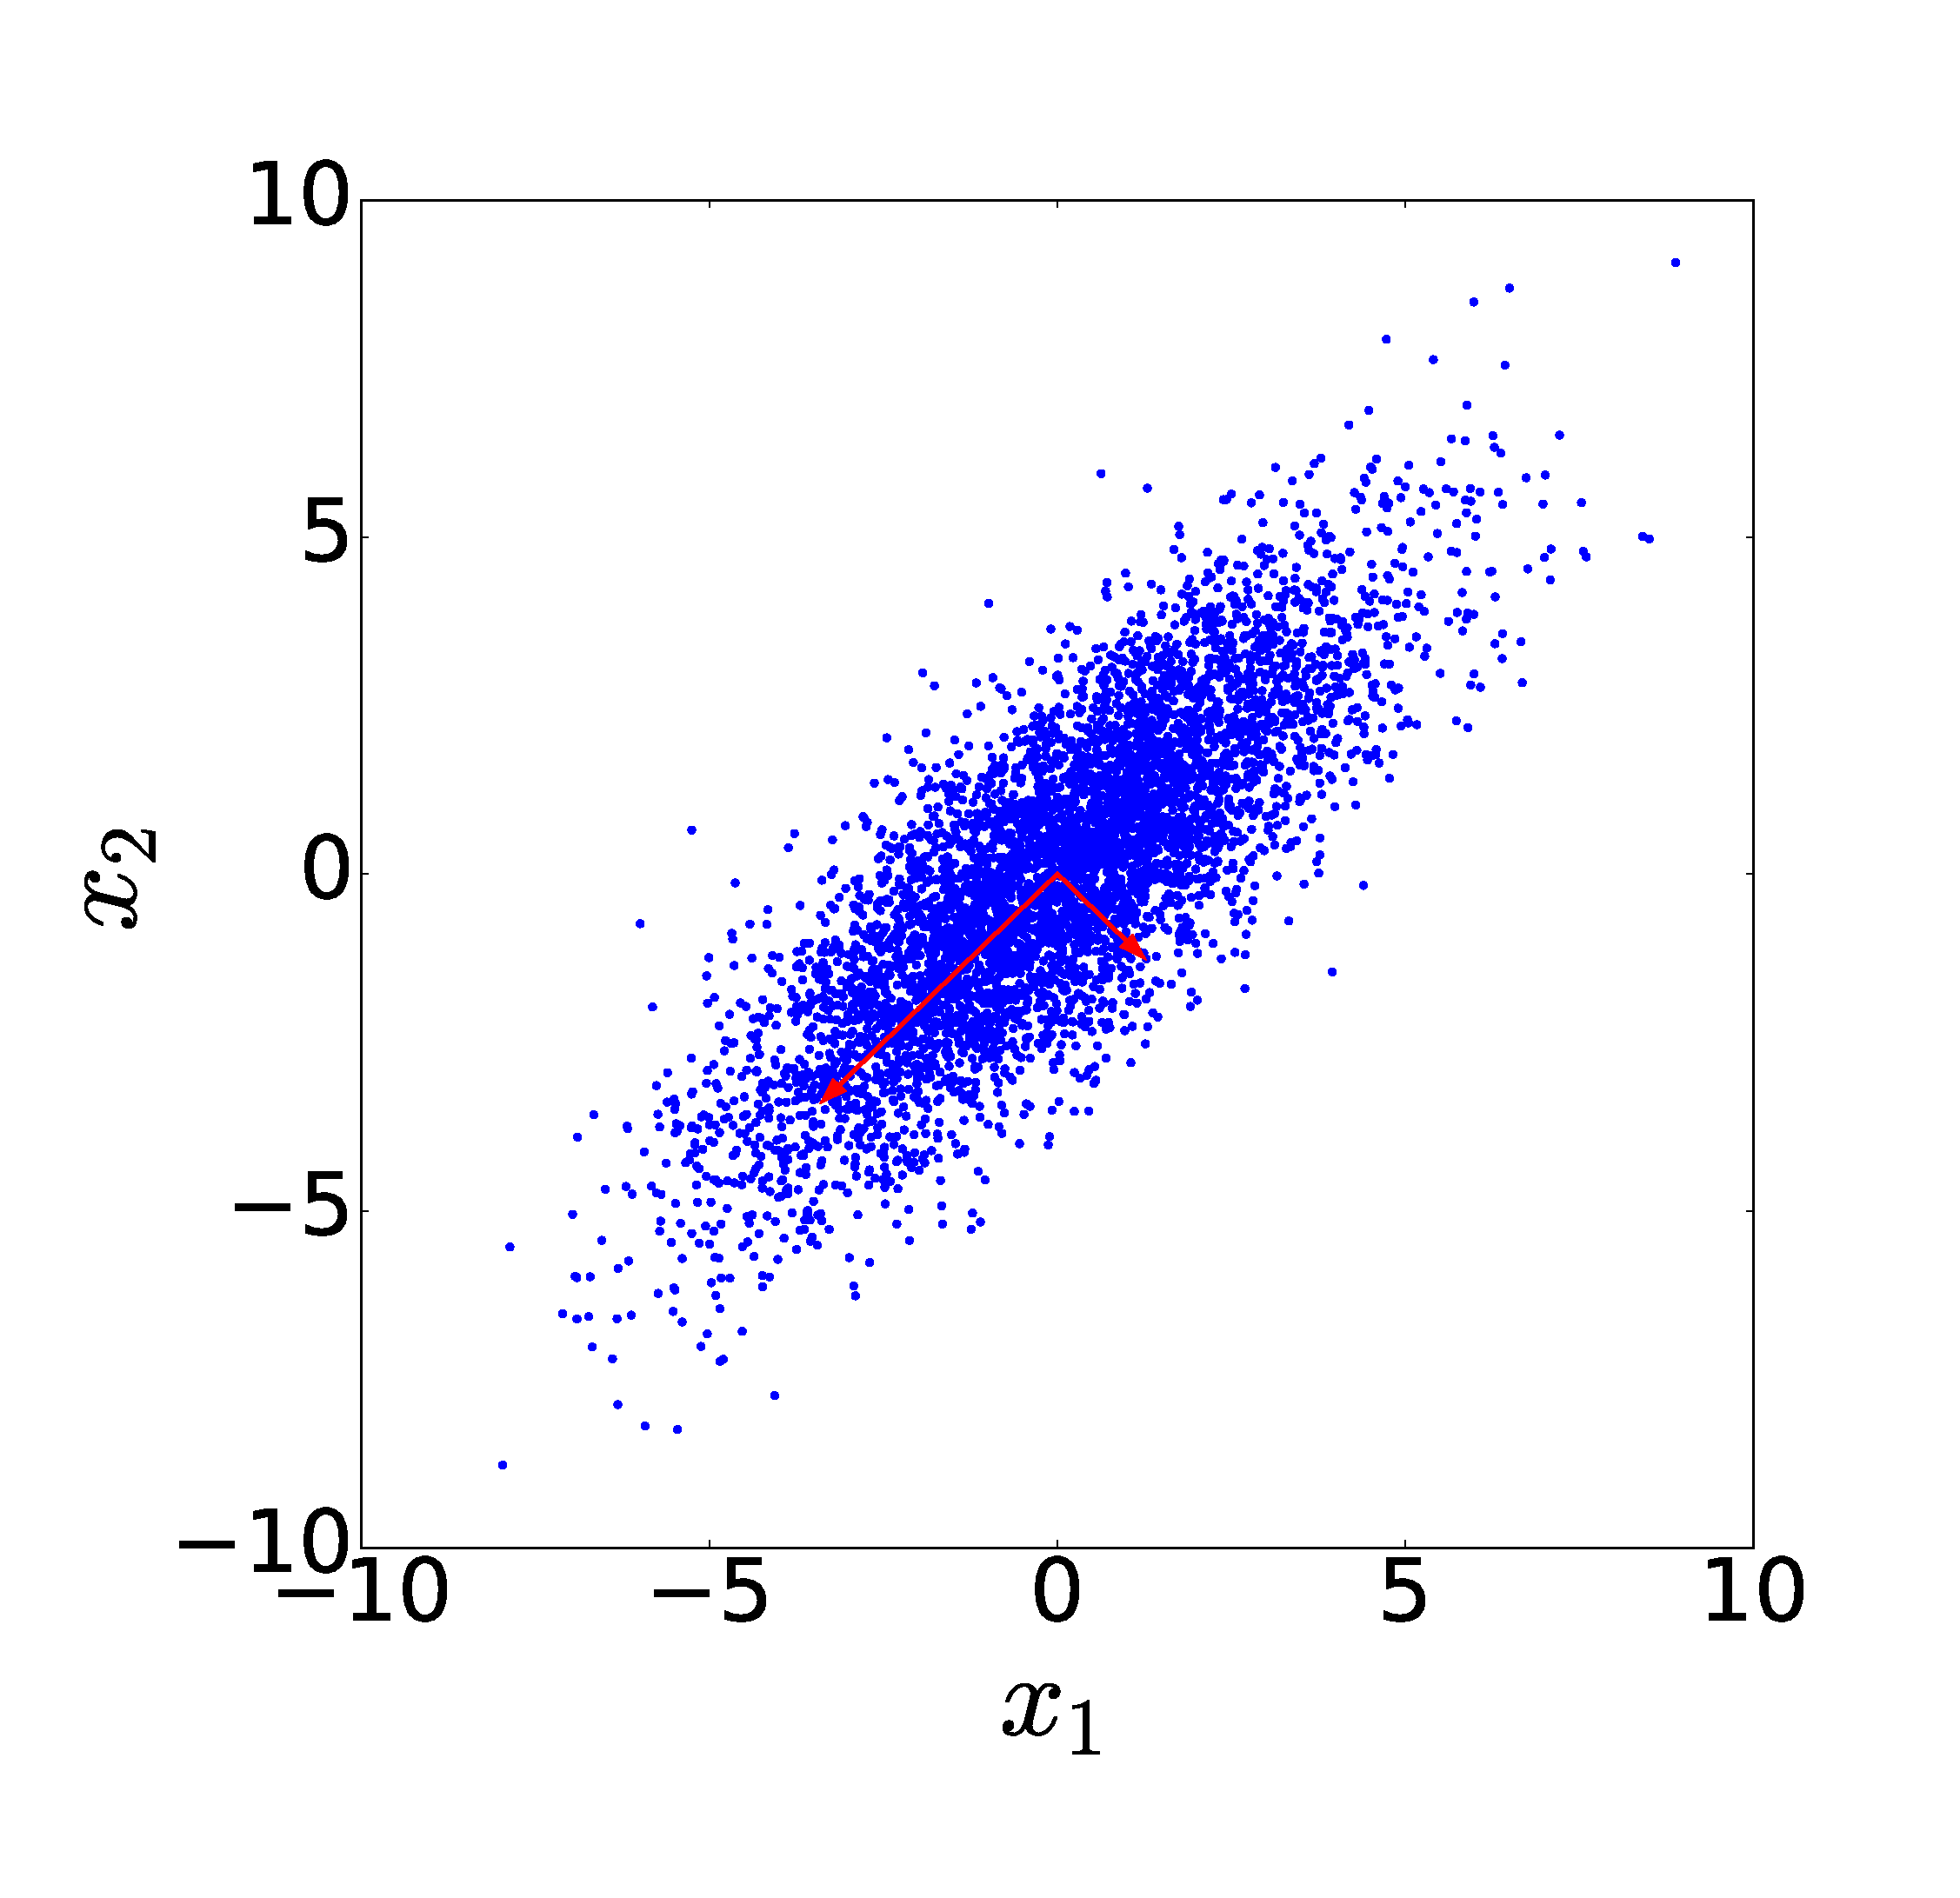
\includegraphics[width=0.8\textwidth]{pca-ex}
  \caption[Example of principal component analysis]{Principal
    components found through PCA on the blue point cloud, scaled by
    singular value. \label{fig:pca-ex}}
\end{figure}

Besides its relative simplicity and ease of implementation, PCA has
one other great strength compared to other dimensionality reduction
methods: it provides an explicit functional form between the input
variables and the output projection in the form of a simple, linear
relationship. In the context of PCA, the principal vectors, which are
some linear combination of the input variables, are precisely the
``best'' new variables to work in. Using the output of the previous
example, we may decide that only the value $x_1 + x_2$ is important
enough to keep, allowing us to reduce our description of the dataset
from $(x_1, x_2) \rightarrow (x_1 + x_2)$. As we will see in the
following section, while more complex methods offer distinct
advantages over PCA, they lack such easily interpretable results.

\subsection{Diffusion Maps \label{sec:dmaps}}

While PCA may be effective in uncovering linear relationships among
input variables, most real-world problems exhibit significant
nonlinearities. This motivates our introduction of Diffusion Maps
(DMAPS), an algorithm designed to address such difficulties. We begin
with a description of the DMAPS' implementation.

The goal of DMAPS is identical to that of PCA: given some dataset
$\{x_1, x_2, \hdots, x_N \}$ with $x_i \in \R^n$, we desire a mapping
of $x_i$ into $y_i$ such that $y_i$ is a low-dimensional embedding of
$x_i$ that captures important characteristics of the original data. We
again stack each datapoint $x_i$ into an $N \times n$ matrix
$X$. DMAPS begins by evaluating a Gaussian kernel between each point,
and storing the results in an $N \times N$ matrix $W$, so that

\begin{align}
  W_{ij} = \exp \left( -\frac{\|x_i - x_j\|^2}{\epsilon^2} \right)
\end{align}

where $\epsilon$ is a parameter which will be discussed below. Note
that $W_{ij} \rightarrow 0$ as the distance between $x_i$ and $x_j$
increases. We then calculate the sum of each row of $W$, and use these
values to construct a new diagonal matrix $D$ with
$D_{ii} = \sum_j W_{ij}$. Finally, we compute $A = D^{-1} W$. As
$A_{ij} \ge 0$ and $\sum_j A_{ij} = 1$, $A$ is a stochastic
matrix. This lends its entries $A_{ij}$ an intuitive interpretation:
if we are performing a random walk from point to point in our dataset,
$A_{ij}$ is the probability that, starting from $x_i$ we will hop next
to $x_j$. Just as $W_{ij}$ decreases when the distance between $x_i$
and $x_j$ grows, so too will $A_{ij}$ decrease, so that the
probability of jumping to nearby points is much greater than the
probability of jumping to distant ones. This concept is illustrated in
Fig.~\ref{fig:dmaps-3pts} for three points.

\begin{figure}
  \centering
  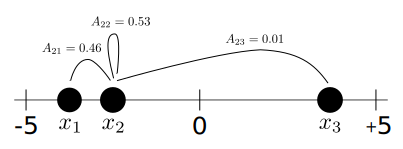
\includegraphics[width=0.8\textwidth]{dmaps-3pts}
  \caption[Illustration of random walk on data]{Probability of
    transitioning from $x_1$ to points $x_2$ and $x_3$ and to
    itself. \label{fig:dmaps-3pts}}
\end{figure}


Having constructed the stochastic matrix $A$, the penultimate step in
the DMAPS algorithm is to perform an eigen-decomposition of
$A$. Numerically, it is helpful to note that $A$ is similar to the
symmetric matrix $\hat{A}$

\begin{align}
  \hat{A} &= D^{1/2}A D^{-1/2} \\
  & = D^{-1/2} W D^{-1/2}
\end{align}

As specialied eigensolvers such as the Lanczos algorithm have been
developed for symmetric matrices, it is best to transform $A$ into
$\hat{A}$, calculate the eigendecomposition, and transform the
eigenvectors of $\hat{A}$ into eigenvectors of $A$ by multiplying by
$D^{-1/2}$. This results in eigenvalues
$\la_0 \ge |\la_1| \ge \cdots \ge |\la_{n-1}|$ with $\la_0 = 1$ and
corresponding eigenvectors $\phi_0, \phi_1, \cdots, \phi_{n-1}$. That
all eigenvalues have absolute value no greater than one is a
consequence of Gershgorin's circle theorem, while the existence of
$\la_0 = 1$ is clear when one considers the eigenvector $v_0 = (1/N,
1/N, \cdots, 1/N)^T$, so that, for any row stochastic matrix $A$, $A
v_0 = \la_0 v_0$. Finally, the low-dimensional map is given by

\begin{align}
  \Phi_t: x_i \rightarrow \begin{bmatrix} \la_1^t \phi_1(i) \\ \la_2^t
    \phi_2(i) \\ \vdots \\ \la_k^t \phi_k(i) \end{bmatrix} \in \R^k
\end{align}

where we have chosen the top $k \ll N$ eigenvectors to embed our data,
and $\phi_j(i)$ represents the $i$th component of $\phi_j$. It is not
immediately clear what the effect of such a mapping is, but there are
two useful characterizations of the DMAPS embeddings that elucidate
its utility. First, letting $y_i = \Phi(x_i)$, we can show that $y_i$
provides the best $k$-dimensional approximation to the so-called
``diffusion distance'' between points. We now detail this connection.

\subsubsection{Diffusion distance}

Returning to our stochastic matrix $A$, say we have a vector
$\Psi_t \in \R^N$ where each entry $\Psi_t(i)$ represents the
probability of finding a random walk at data point $i$ at step $t$ of
the walk (so $\sum_j \Psi_t(j) = 1$ and $\Psi_t(j) \ge 0$). In other
terms, $\Psi_t(j) = p(r_t = x_j)$ where $r_i$ is the position of the
random walk at iteration $i$. We then have that

\begin{align}
  \Psi_t^T = \Psi_0^T A^t
\end{align}

to see this, note that

\begin{align*}
  \Psi_t^T A = \big( &\sum_i \Psi_t(i) A_{i1},\; \sum_i
                         \Psi_t(i) A_{i2},\; \dots,\; \sum_i \Psi_t(i) A_{iN} \big) \\
             = \bigg( &\sum_i p(r_{t+1} = x_1 | r_t = x_i)p(r_t = x_i) , \\
             & \sum_i p(r_{t+1} = x_2 | r_t = x_i)p(r_t = x_i), \\
             & \dots, \\
                     & \sum_i p(r_{t+1} = x_N | r_t = x_i)p(r_t = x_i)
                       \bigg) \\
  = \bigg( & p(r_{t+1} = x_1), \;p(r_{t+1} = x_2), \; \dots, \;
             p(r_{t+1} = x_N) \bigg) \\
  = & \Psi_{t+1}
\end{align*}

so by multiplying $\Psi_0$ by $A^t$, we march our random walk forward
$t$ steps. In the limit of infinite steps, we find that the
probability distribution becomes stationary, so further applications
of $A$ do not change the probability of being at a particular
point. We will call this stationary distribution $\Psi_*$, and find
that

\begin{align}
  \Psi_*^T &= \lim_{t \rightarrow \infty} \Psi_0^T A^t \\
           &= \Psi_*^T A
\end{align}

Thus $\Psi_*$ is the right eigenvector of $A$ with eigenvalue one. By
inspection, its entries will be $\Psi_*(i) = \frac{d_i}{\sum_j d_j}$
where $d_i = \sum_i A_{ij}$.

We now define the diffusion distance at time $t$ between points $x$
and $y$ to be

\begin{align}
  D^2_t(x_i, x_j) &= \| p(r_t = x_i| \cdot) - p(r_t = x_j | \cdot) \|^2_{1/\Psi_*} \\
                  &= \sum_k \frac{A^t_{ki} - A^t_{kj}}{\Psi_*(k)} \\
\end{align}

Now, denoting the right eigenvectors of $A$ as $\psi_i$, we have
$A^t_{ij} = \sum_k \la_k^t \phi_k(i) \psi_k(j)$ by the spectral
decomposition of $A$. Substituting this into the equation above gives

\begin{align}
  D^2_t(x_i, x_j) &= \sum_{k=1}^{N-1} \la_k^t \left( \phi_k(i) -
                    \phi_k(j) \right)^2 \\
\end{align}

where we omit $k=0$ which corresponds to the constant
eigenvector. Finally, we see that this diffusion distance between
points is approximated by the Euclidean distance between $y_i$ and
$y_j$. As we have chosen the largest $k$ eigenvalues to include in
$y_i$, and assuming the magnitude of the eigenvalues decays quickly
after $\la_k$, we see that

\begin{align}
  D^2_t(x_i, x_j) & \approx \sum_{k=1}^{k} \la_k^t \left( \phi_k(i) -
                    \phi_k(j) \right)^2 \\
  & = \| y_i - y_j \|^2
\end{align}

This provides an interesting probabilisitic interpretation to the
DMAPS embedding. We now turn to a geometric view of the algorithm.

\subsubsection{Eigenfunctions of operators}

Besides embedding points based on their approximate diffusion
distances, DMAPS also provides a parameterization of the manifold on
which the data reside by yielding approximate eigenfunctions of
diffusion operators defined on the manifold. We assume that our data
have been sampled from an underlying manifold $\chi$ with some density
$p(x)$. Essentially, as the number of points tends to infinity and our
$\epsilon$ scaling term tends to zero, the resulting stochastic matrix
$A$ approximates certain differential operators depending on the value
of $\alpha$ in the algorithm. These are given below

\begin{equation}
\begin{aligned}
  \alpha &= 0: &&\frac{(I - A)}{\epsilon} \phi = \Delta \phi + 2
    \nabla \phi \cdot \frac{\nabla p}{p} \\
  \alpha &= 1/2: &&\frac{(I - A)}{\epsilon} \phi = \Delta \phi +
    \nabla \phi \cdot \frac{\nabla p}{p} \\
  \alpha &= 1: &&\frac{(I - A)}{\epsilon} \phi = \Delta \phi
\end{aligned}
\end{equation}

The eigenvectors of $A$ will then approximate the eigenfunctions of
the corresponding operator. In particular, we see that with the choice
$\alpha = 1$, we recover the Laplace-Beltrami operator on our
manifold. As such, the resulting eigenvectors will be influenced only
by the geometry of the manifold and not by our sampling density on
it. However, if our data is uniformly sampled so that $p(x) = c$, all
values of $\alpha $ yield the same result.

We illustrate this result with an analytically tractable example for
which the manifold is a simple rectangle, $\chi = [0, L_x] \times [0,
L_y]$ where $L_x$ and $L_y$ are the lengths of the rectangle along the
$x$ and $y$ axes. We wish to find the eigenfunctions of the Laplace
operator over the rectangle with homogenous Neumann boundary
conditions. That is, we want to find functions $f$ such that $\Delta f
= \lambda f$ and $\frac{\partial f}{\partial x}\Big|_{x=0,L_x}
=\frac{\partial f}{\partial y}\Big|_{y=0,L_y} = 0$. We solve this
problem using separation of variables to obtain

\begin{align}
  f_{ij} = \cos\left(\frac{i \pi x}{L_x}\right) \cos\left(\frac{j \pi y}{L_y}\right) \quad
  \mathrm{and} \quad \lambda_{ij} = -\left( \left(\frac{i \pi
  }{L_x}\right)^2 + \left(\frac{j \pi}{L_y}\right)^2 \right)
\end{align}

Assigning $L_x = \frac{5}{2}$ and $L_y = 1$ and ordering these eigenpairs by
increasing $|\lambda_{ij}|$, we see that the first few eigenfunctions
will be

\begin{itemize}
\item $\lambda_{10} = -\left(\frac{2 \pi}{5}\right)^2$ with $f_{10} =
  \cos \left(\frac{2 \pi x}{5} \right)$
\item $\lambda_{20} = -\left(\frac{4 \pi}{5}\right)^2$ with $f_{20} =
  \cos \left(\frac{4 \pi x}{5} \right)$
\item $\lambda_{01} = -\pi^2$ with $f_{01} =
  \cos \left( \pi y \right)$
\end{itemize}

The key insight is that the maps $x \rightarrow f_{10} (x)$ and
$y \rightarrow f_{01} (y)$ are bijections from the $x$ and $y$ axes
onto eigenfunctions of the diffusion operator. Thus, instead of
describing points on our rectangular manifold by their $(x,y)$
coordinates, they could equivalently be specified by values of
$(f_{10}, f_{01})$. Although $x$ and $y$ may be a more natural way of
parameterizing the rectangle, in high-dimensional, nonlinear datasets,
this parameterization is unknown. In these cases, we turn to DMAPS to
provide an approximation to these eigenfunctions which, as we have
just seen, will parameterize the hidden manifold our data lie on. This
is the essence of the geometric perspective of DMAPS.

\subsubsection{Examples}

We now provide numerical examples of DMAPS' behavior on simple
datasets to help build an intuitive understanding of its
performance. In all cases, our manifold will be the simple rectangle
described above, with side lengths $L_x = \frac{5}{2}$ and $L_y =
1$. We also fix the number of points to $N = 4000$. Initially we
sample uniformly at random over the rectangle, and then apply the
DMAPS algorithm~\ref{alg:dmaps} to the resulting set of points
$(x_i, y_i)$ $i = 1, \dots, N$. In Fig.~\ref{fig:dmaps-comp} we
compare the numerical results to the theoretical eigenfunctions we
derived in the previous section. The agreement is good, and as
expected, $\phi_1$ and $\phi_3$ parameterize $x$ and $y$
respectively.

\begin{figure}
  \centering
  \begin{subfigure}[t]{0.45\linewidth}
    \centering
    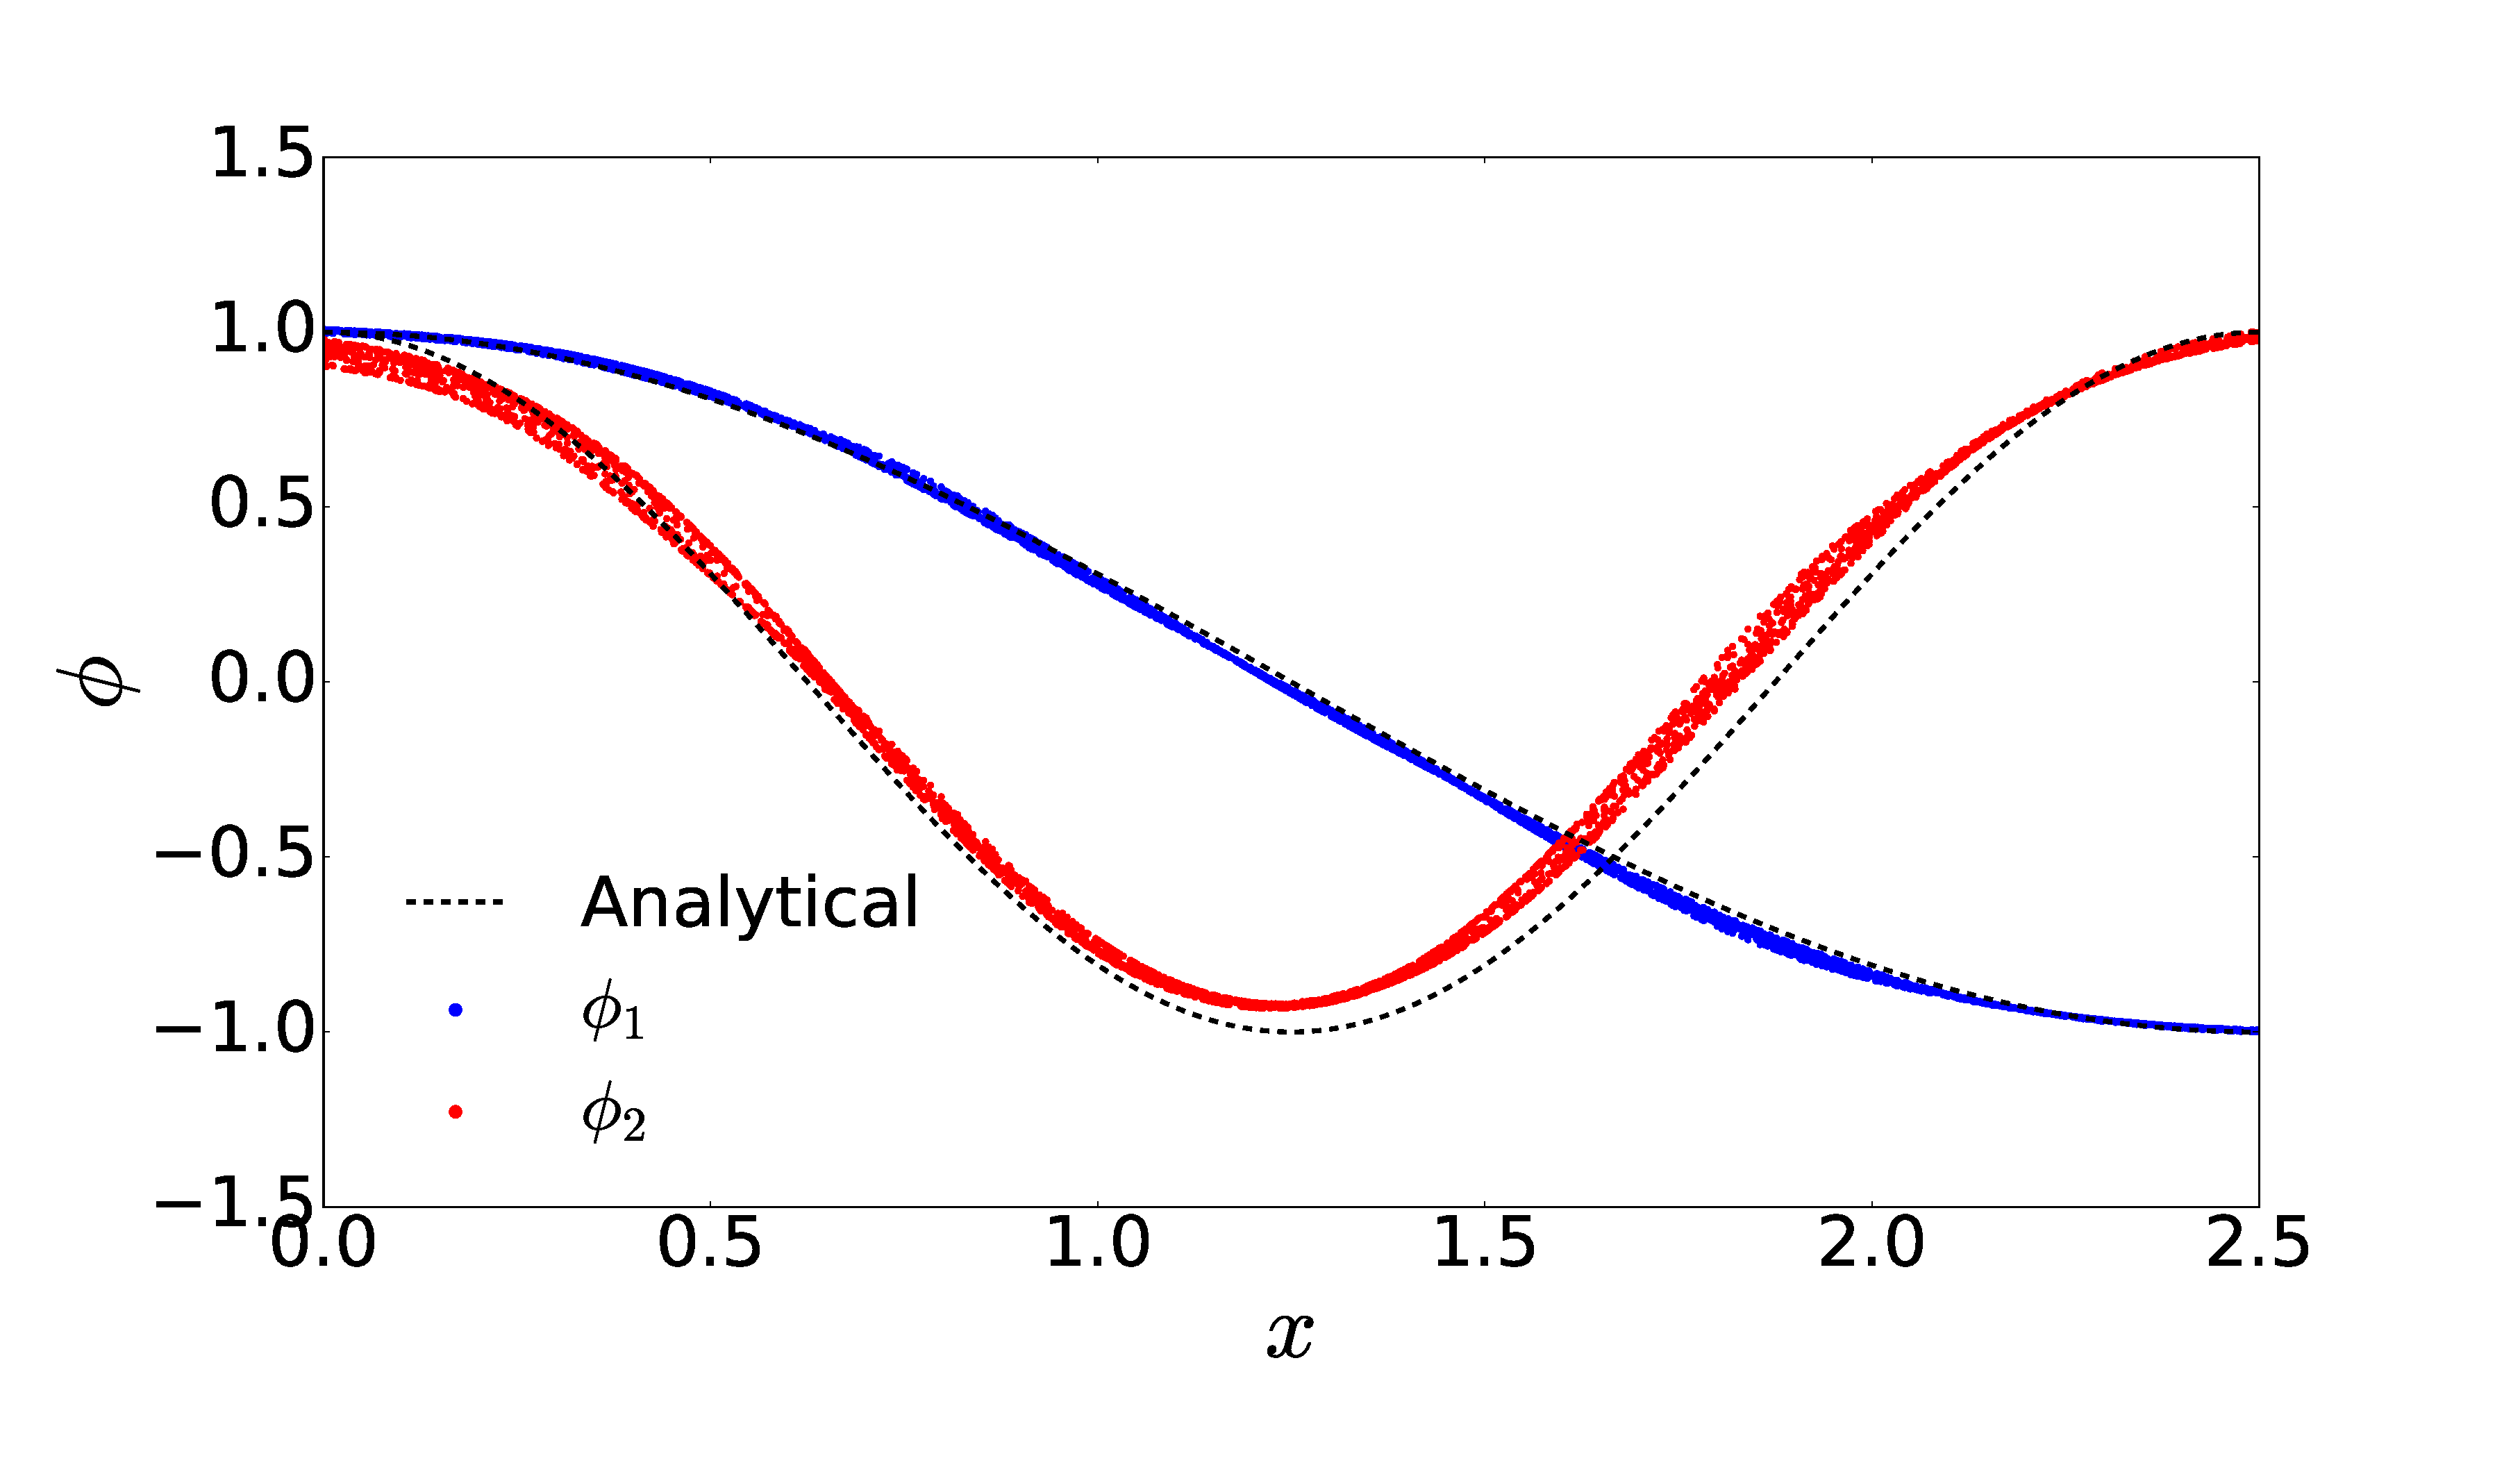
\includegraphics[width=\linewidth]{dmaps-comp-x}
    \subcaption{Comparison of numerical and analytical results for
      $\phi_1 \approx f_{10}$ and $\phi_2 \approx f_{20}$, both of
      which parameterize the $x$ direction.}
  \end{subfigure}
  % \hspace{0.5cm}
  \begin{subfigure}[t]{0.45\linewidth}
    \centering
    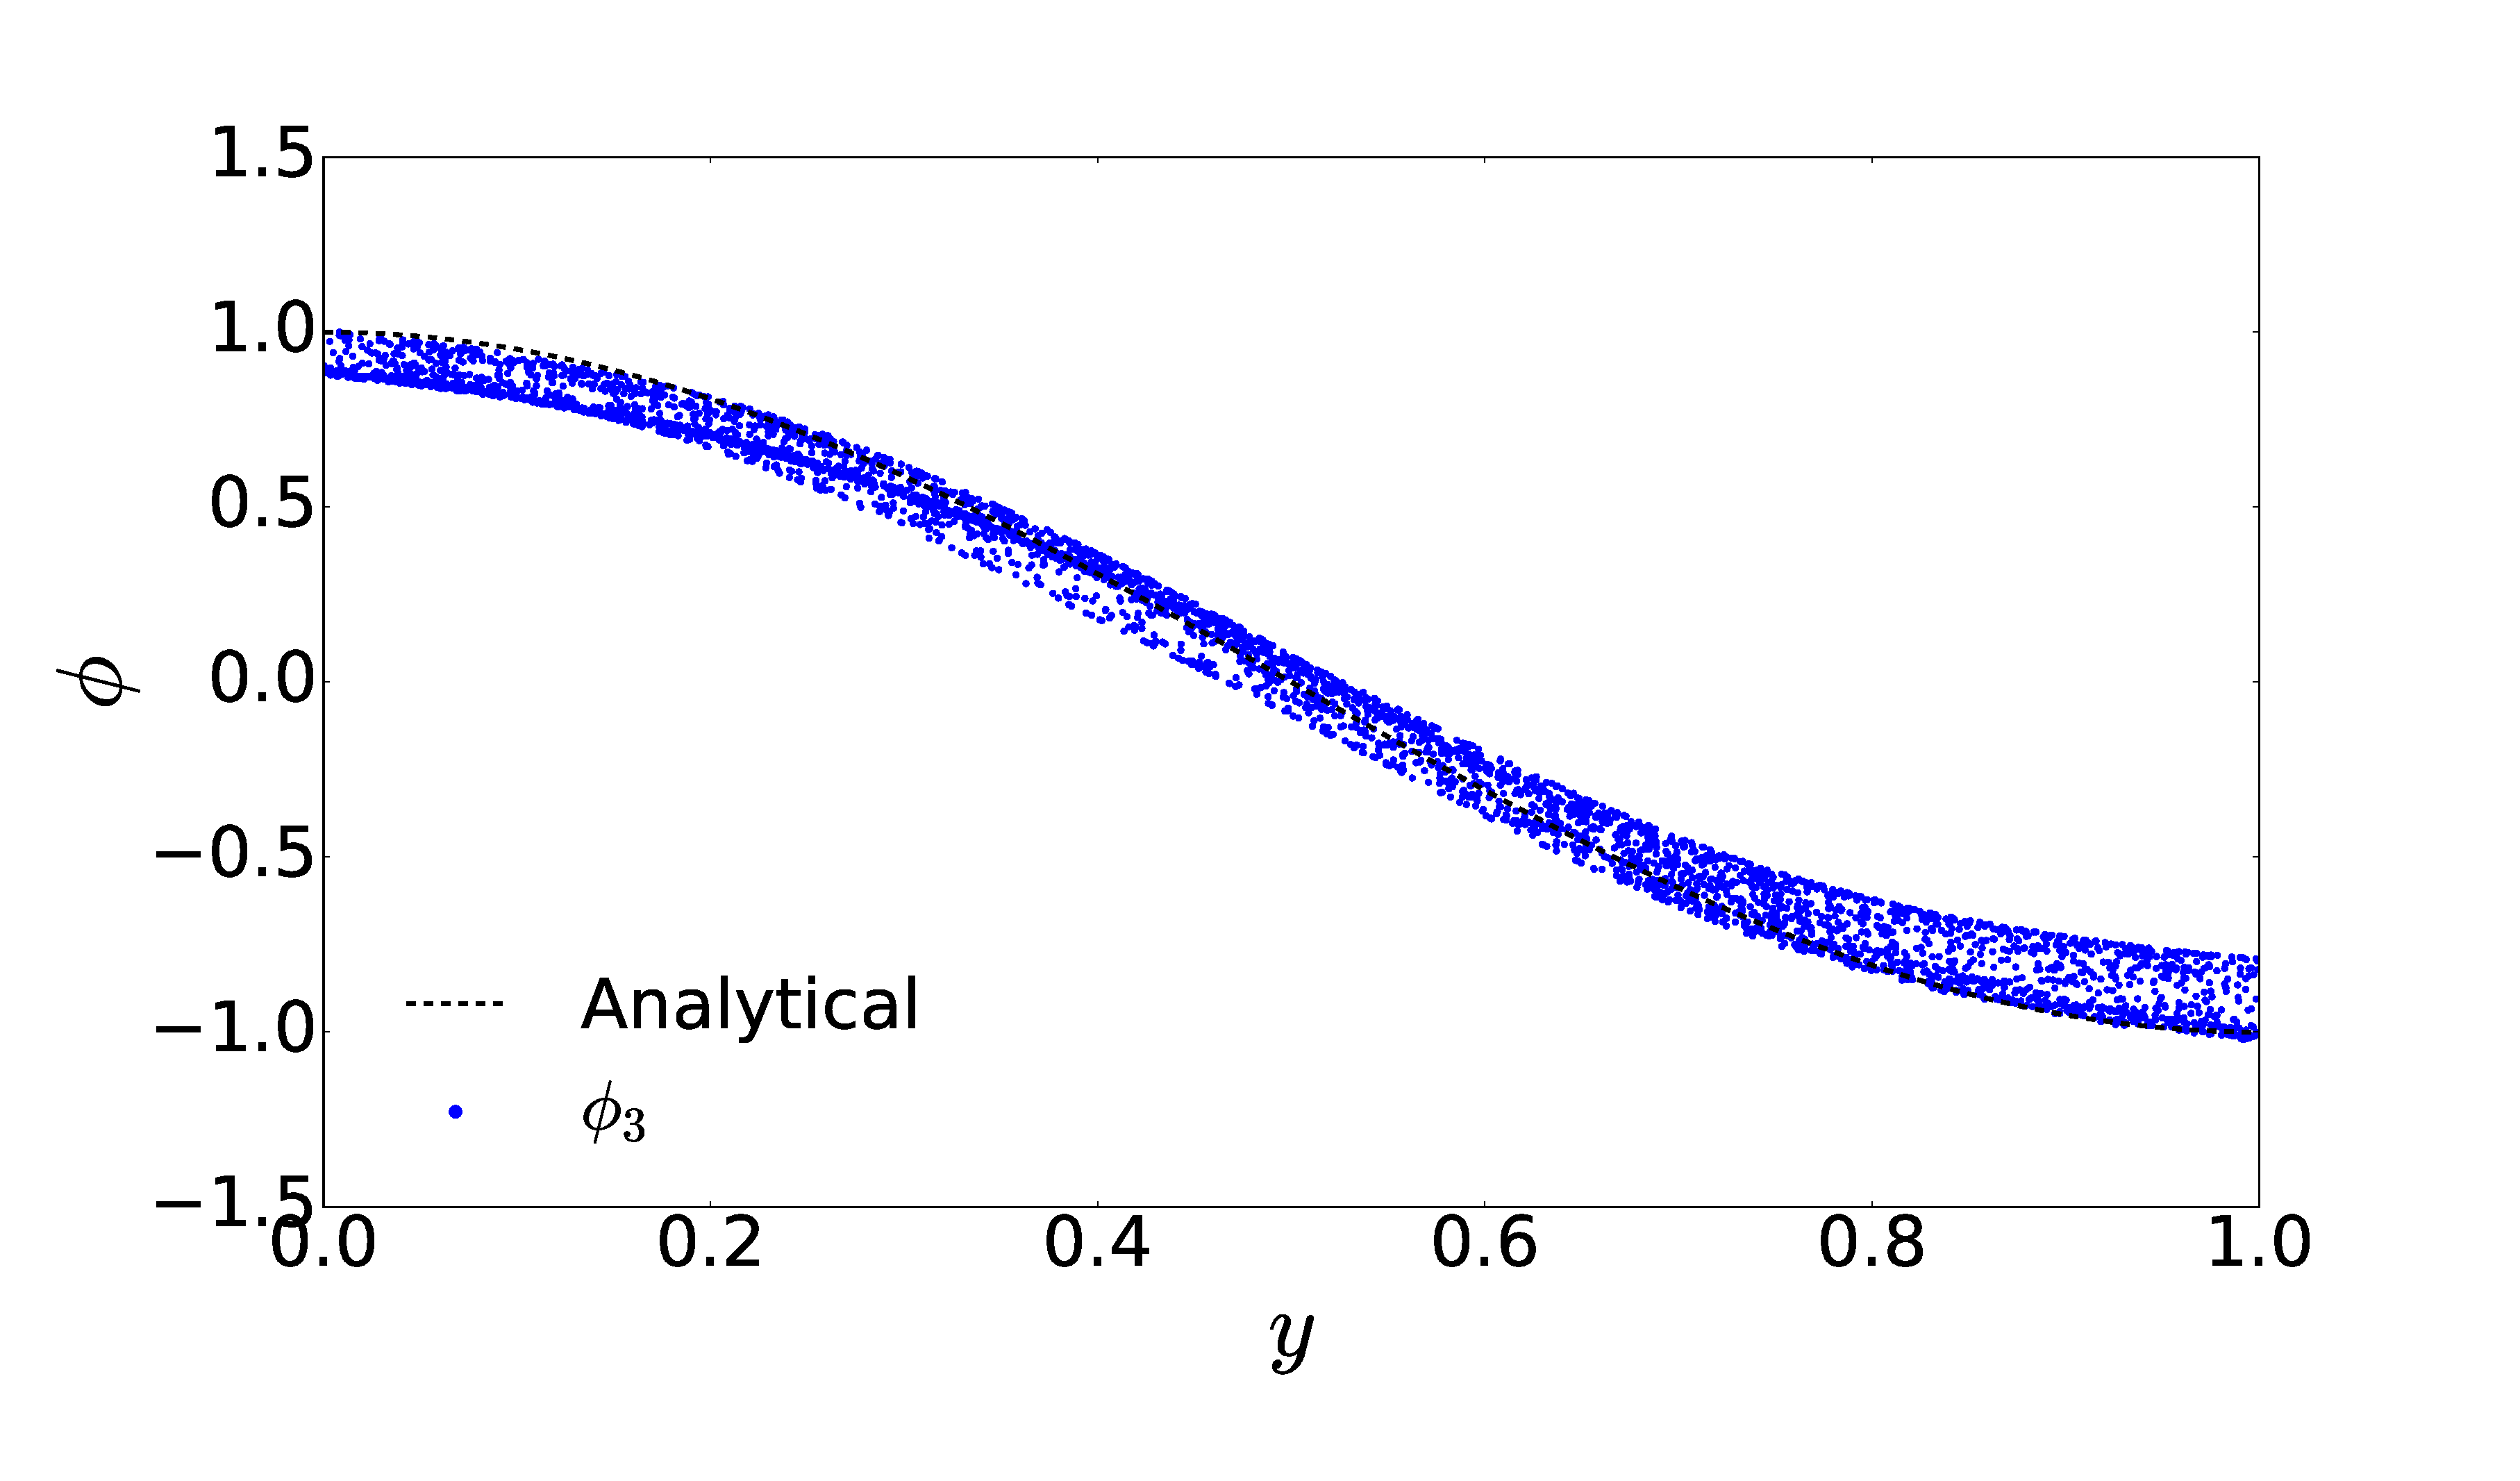
\includegraphics[width=\linewidth]{dmaps-comp-y}
    \subcaption{Comparison of numerical and analytical results for
      $\phi_3 \approx f_{01}$ which parameterizes the $y$ direction.}
  \end{subfigure}
  \caption[Example of DMAPS' parameterization of
  rectangle]{ \label{fig:dmaps-comp} }
\end{figure}

\begin{figure}
  \centering
  \begin{subfigure}[t]{0.45\linewidth}
    \centering
    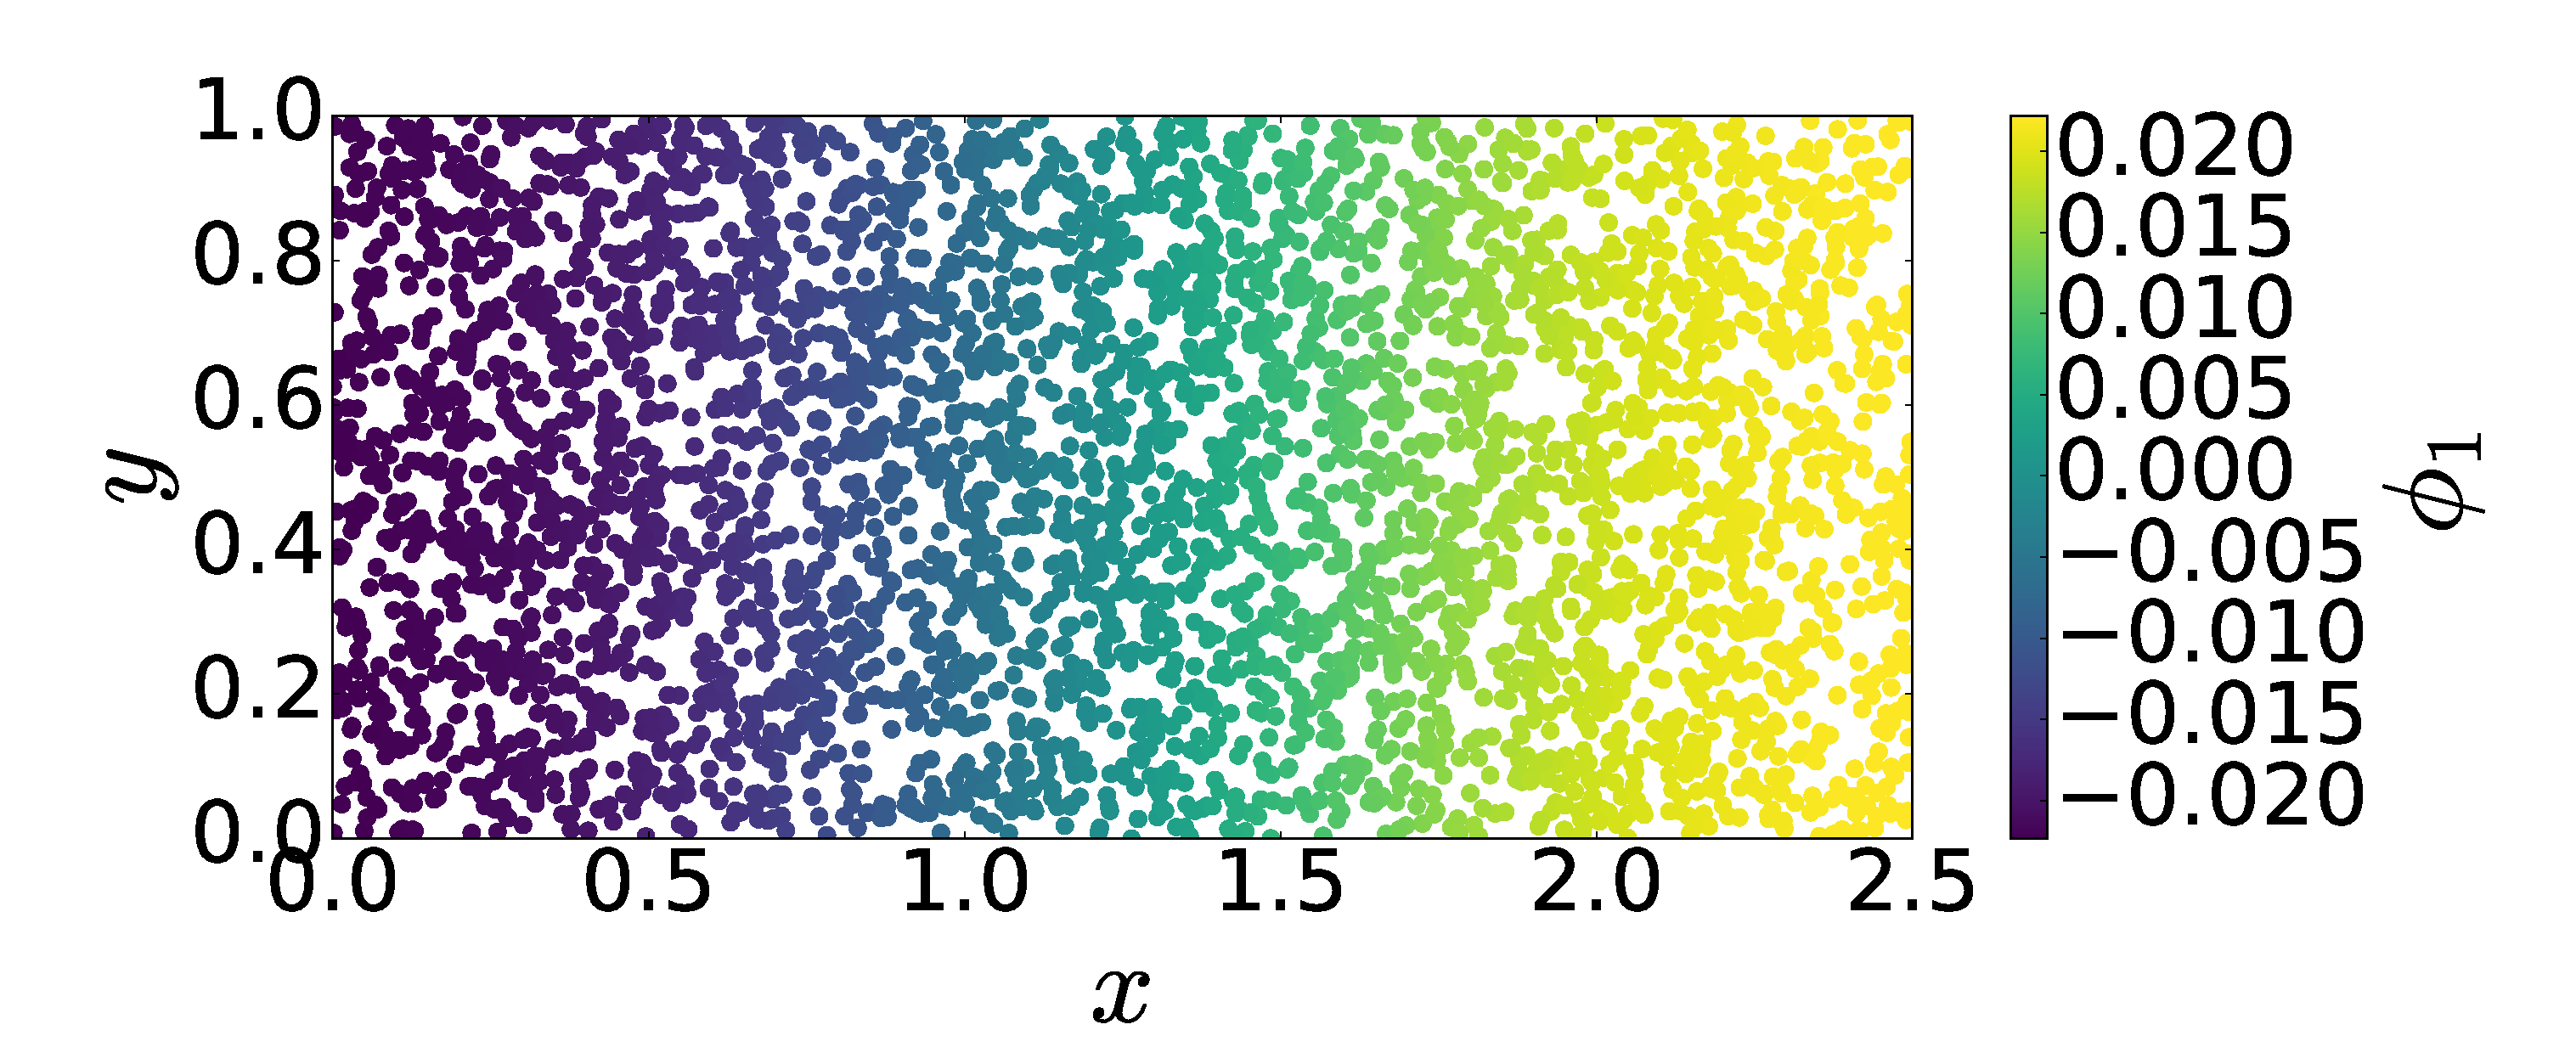
\includegraphics[width=\linewidth]{dmaps-x}
    \subcaption{Coloring the dataset by $\phi_1$, showing that
      $\phi_1$ changes in the $x$ direction.}
  \end{subfigure}
  % \hspace{0.5cm}
  \begin{subfigure}[t]{0.45\linewidth}
    \centering
    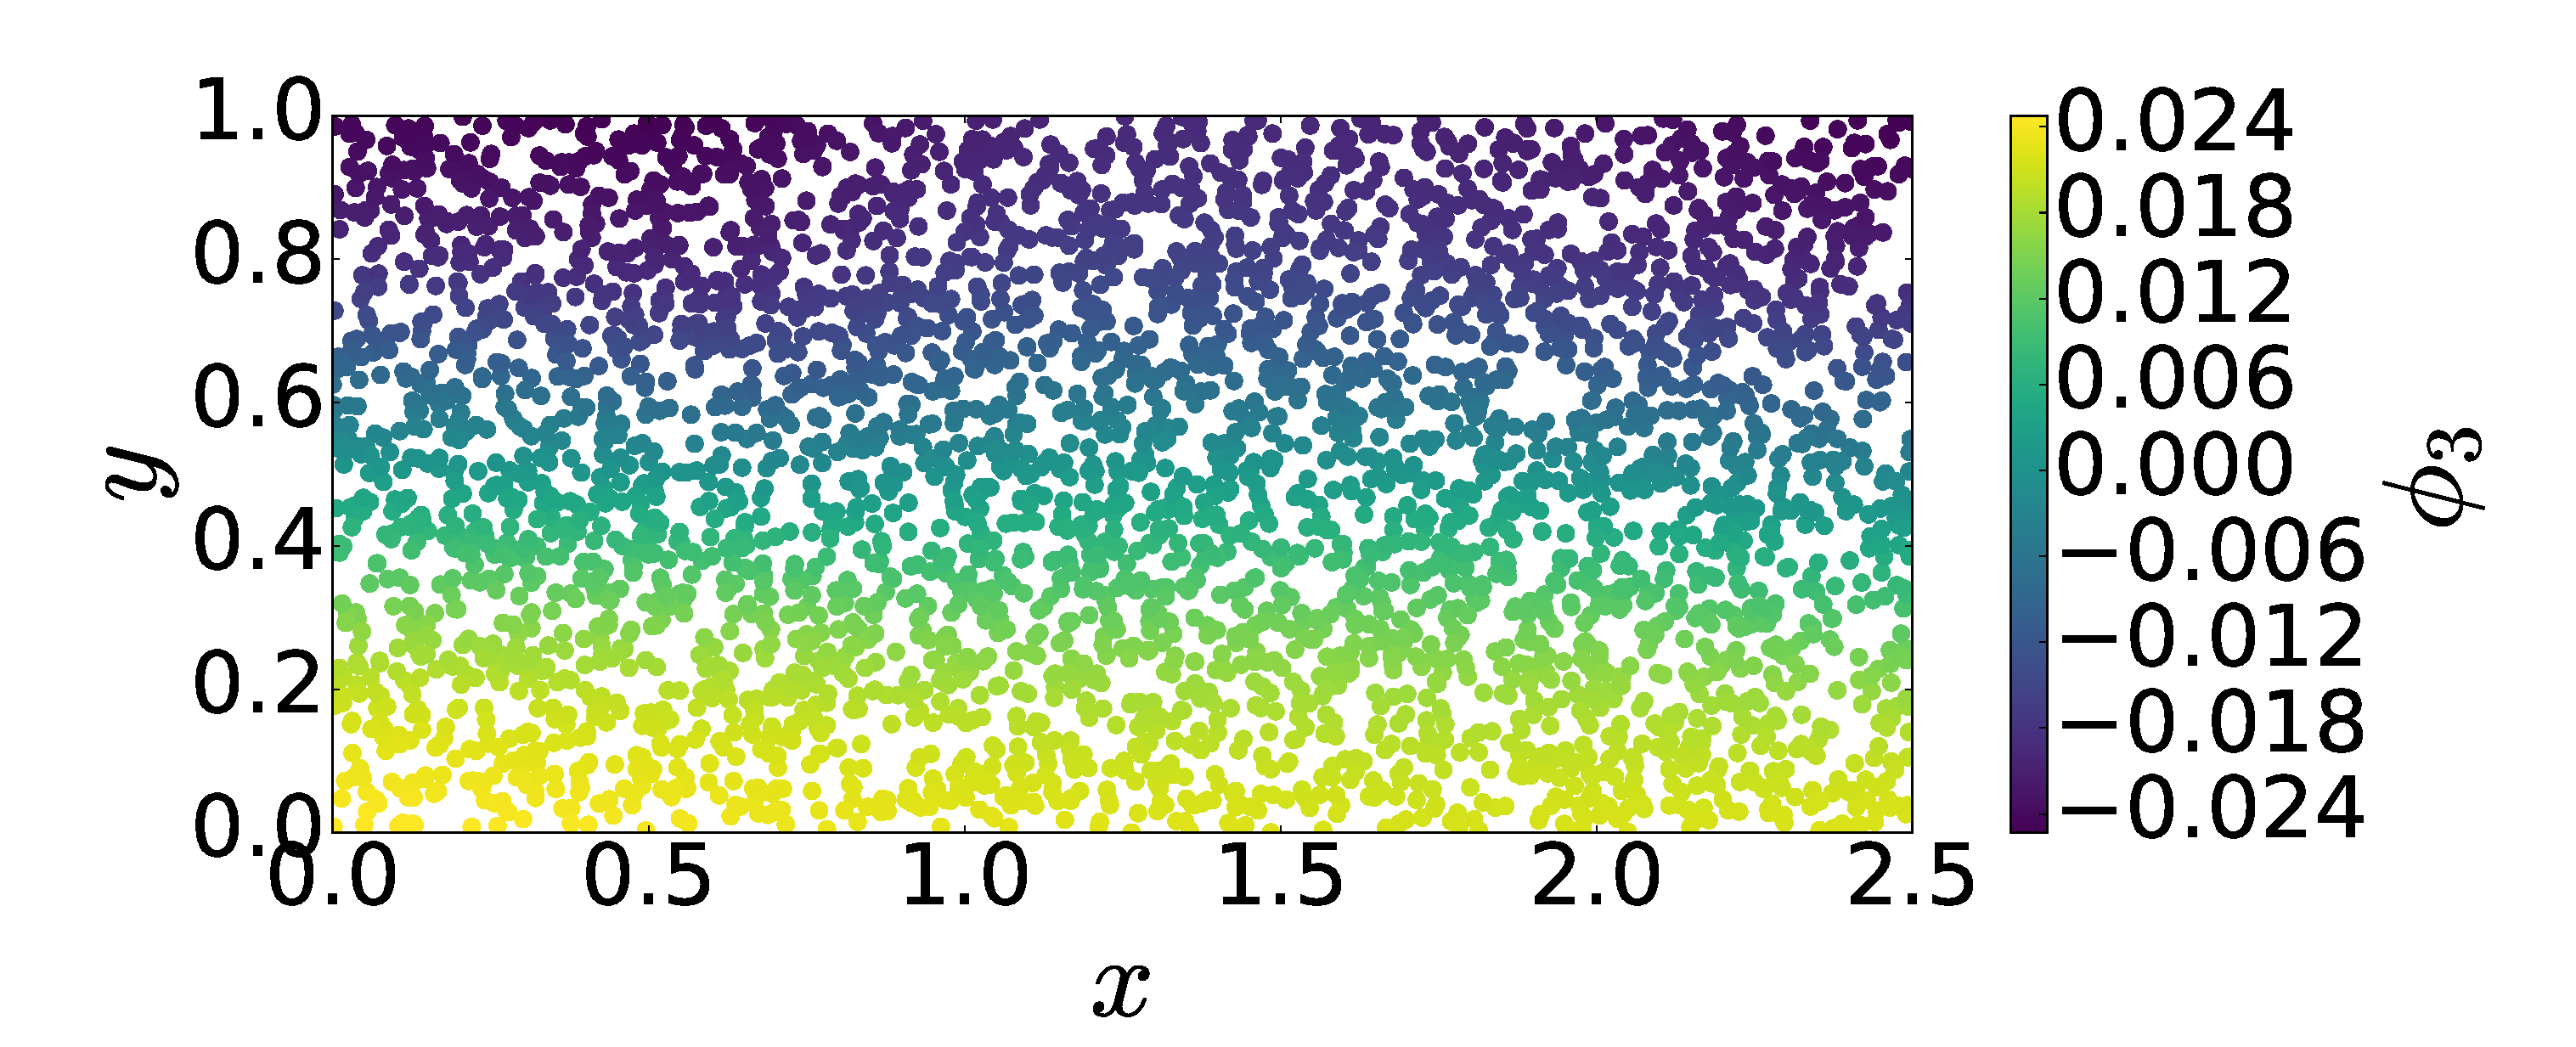
\includegraphics[width=\linewidth]{dmaps-y}
    \subcaption{Coloring the dataset by $\phi_3$, showing that
      $\phi_3$ changes in the $y$ direction.}
  \end{subfigure}
  \caption[Comparison of analytical and numerical DMAPS results]{ \label{fig:dmaps-xy} }
\end{figure}

However, if the density of our points is nonuniform over the rectangle
as shown in Fig.~\ref{fig:dmaps-nonun-data}, the output of algorithm
~\ref{alg:dmaps-unnorm} will be affected by the particular
distribution of points. On the other hand, ~\ref{alg:dmaps} will
continue to approximate eigenfunctions of $\nabla
f$. Fig.~\ref{fig:dmaps-nonun-phi} confirms this behavior.

\begin{figure}
    \centering
    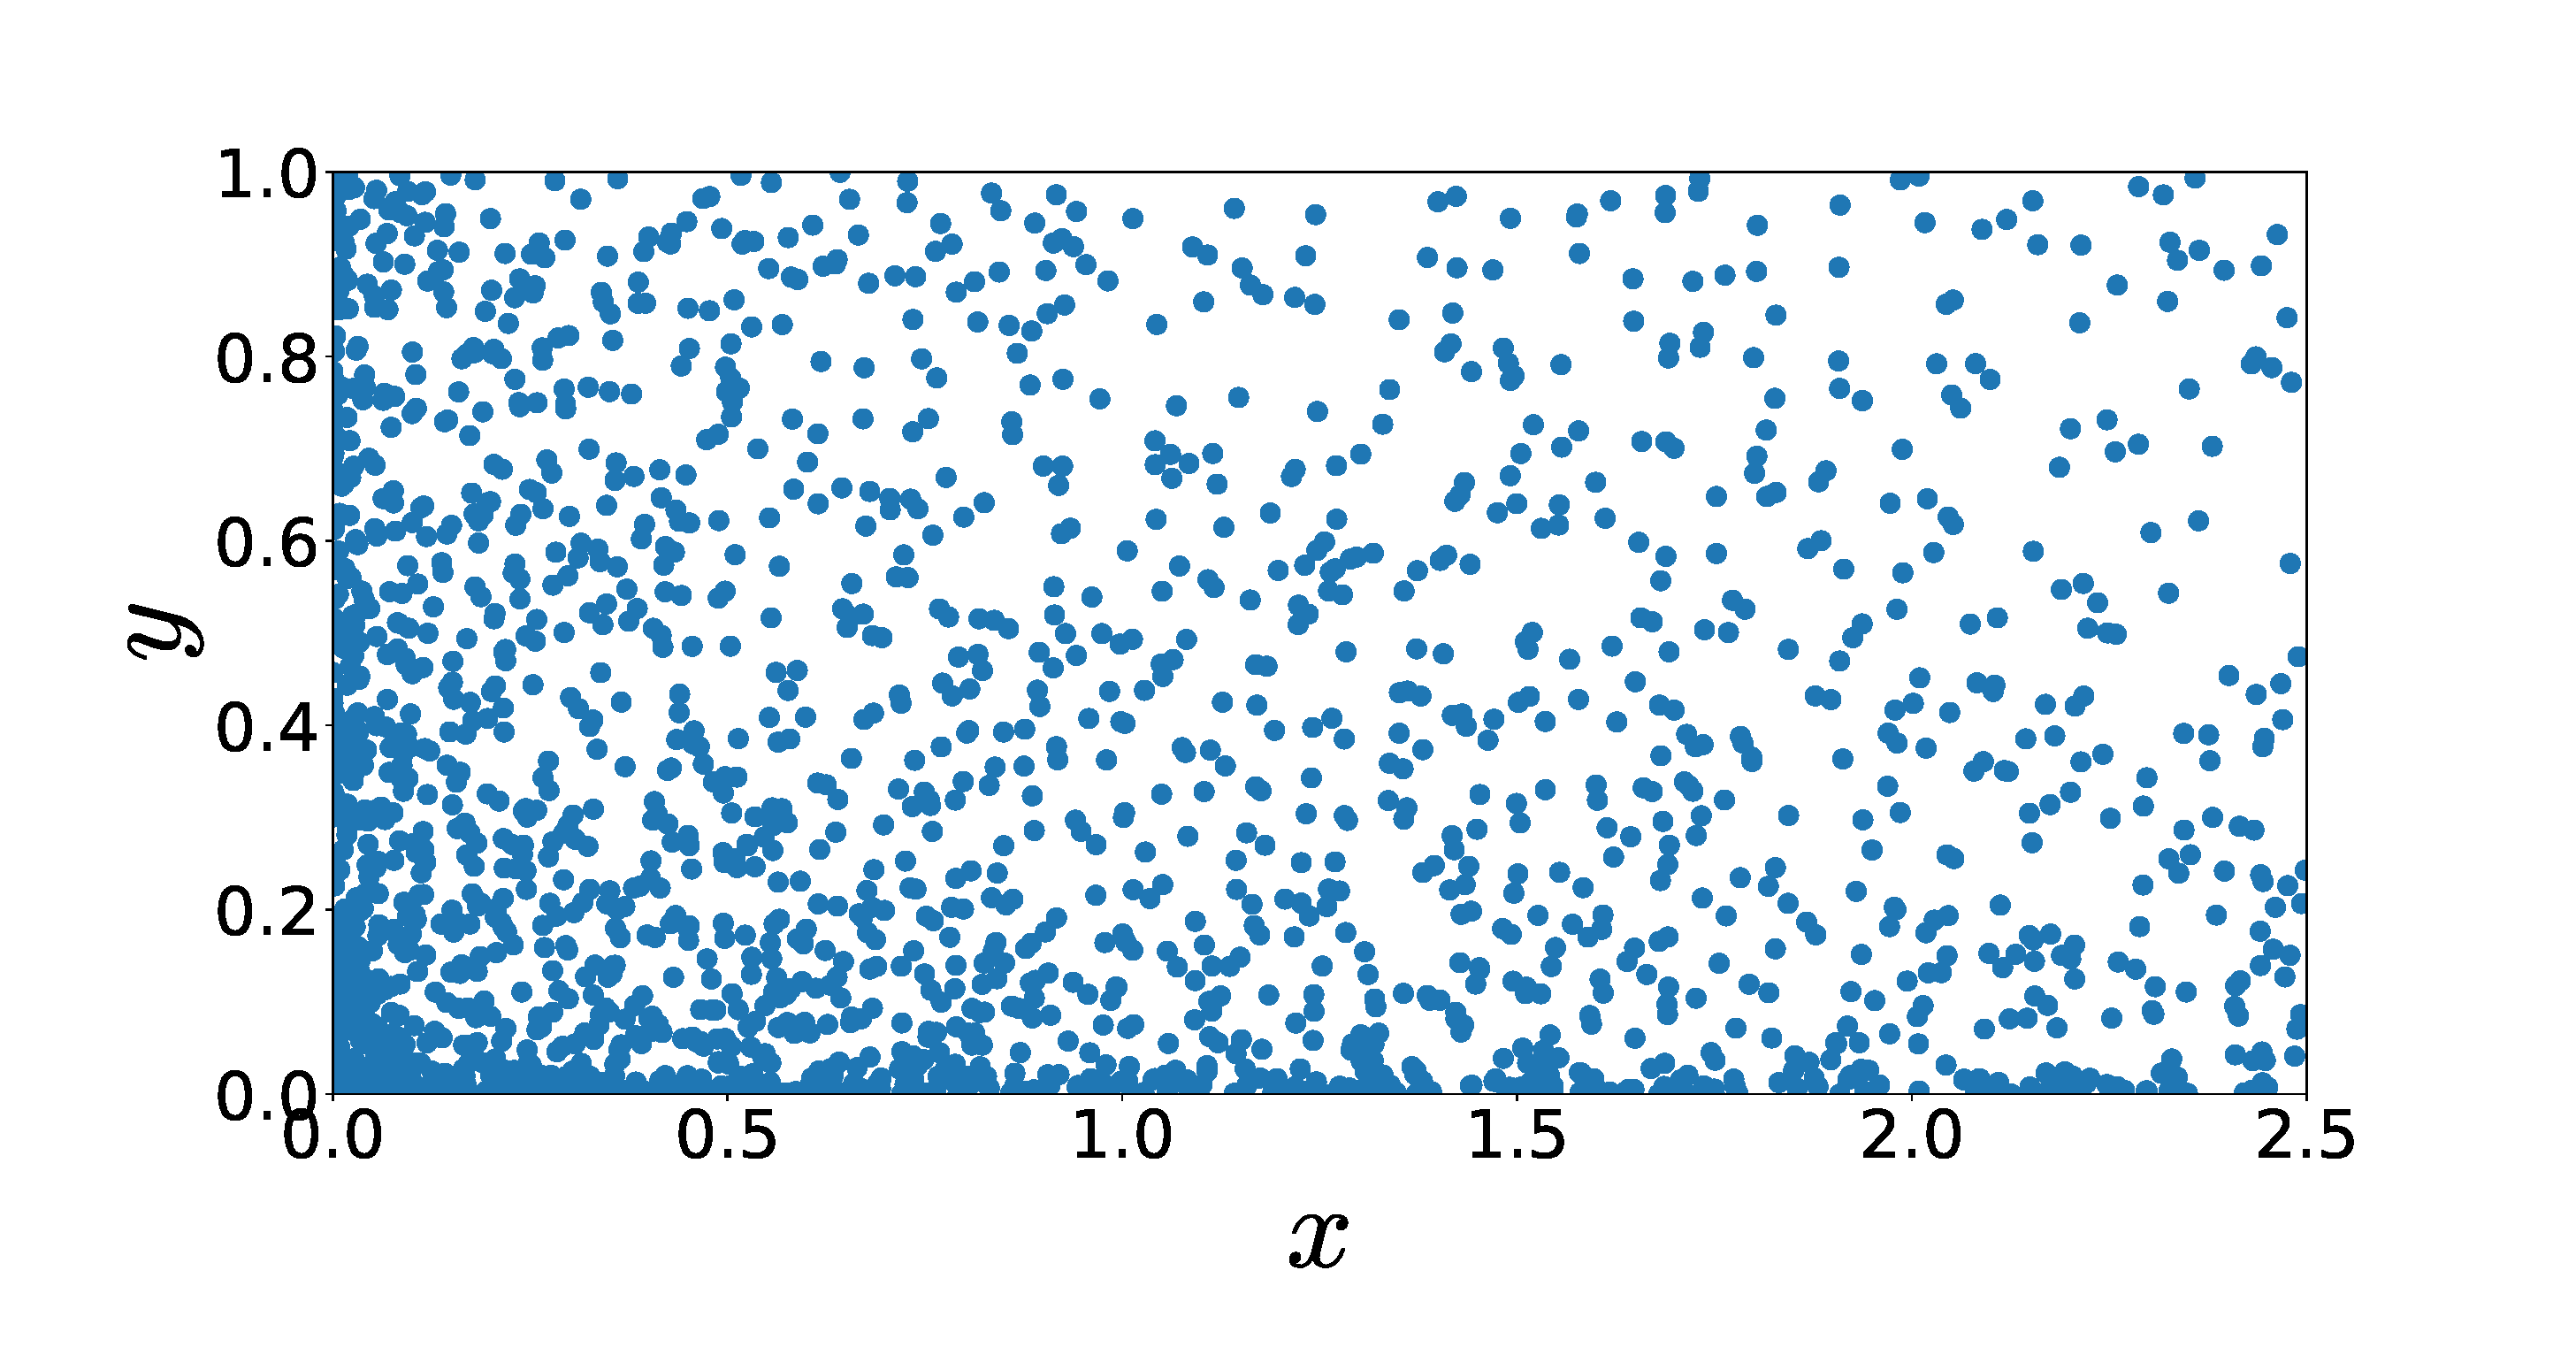
\includegraphics[width=0.9\linewidth]{data-non-y-x}
    \caption[Data with nonuniform density]{Data sampled nonuniformly over the
      rectangle. \label{fig:dmaps-nonun-data} }
\end{figure}


\begin{figure}
  \centering
  \begin{subfigure}[t]{0.45\linewidth}
    \centering
    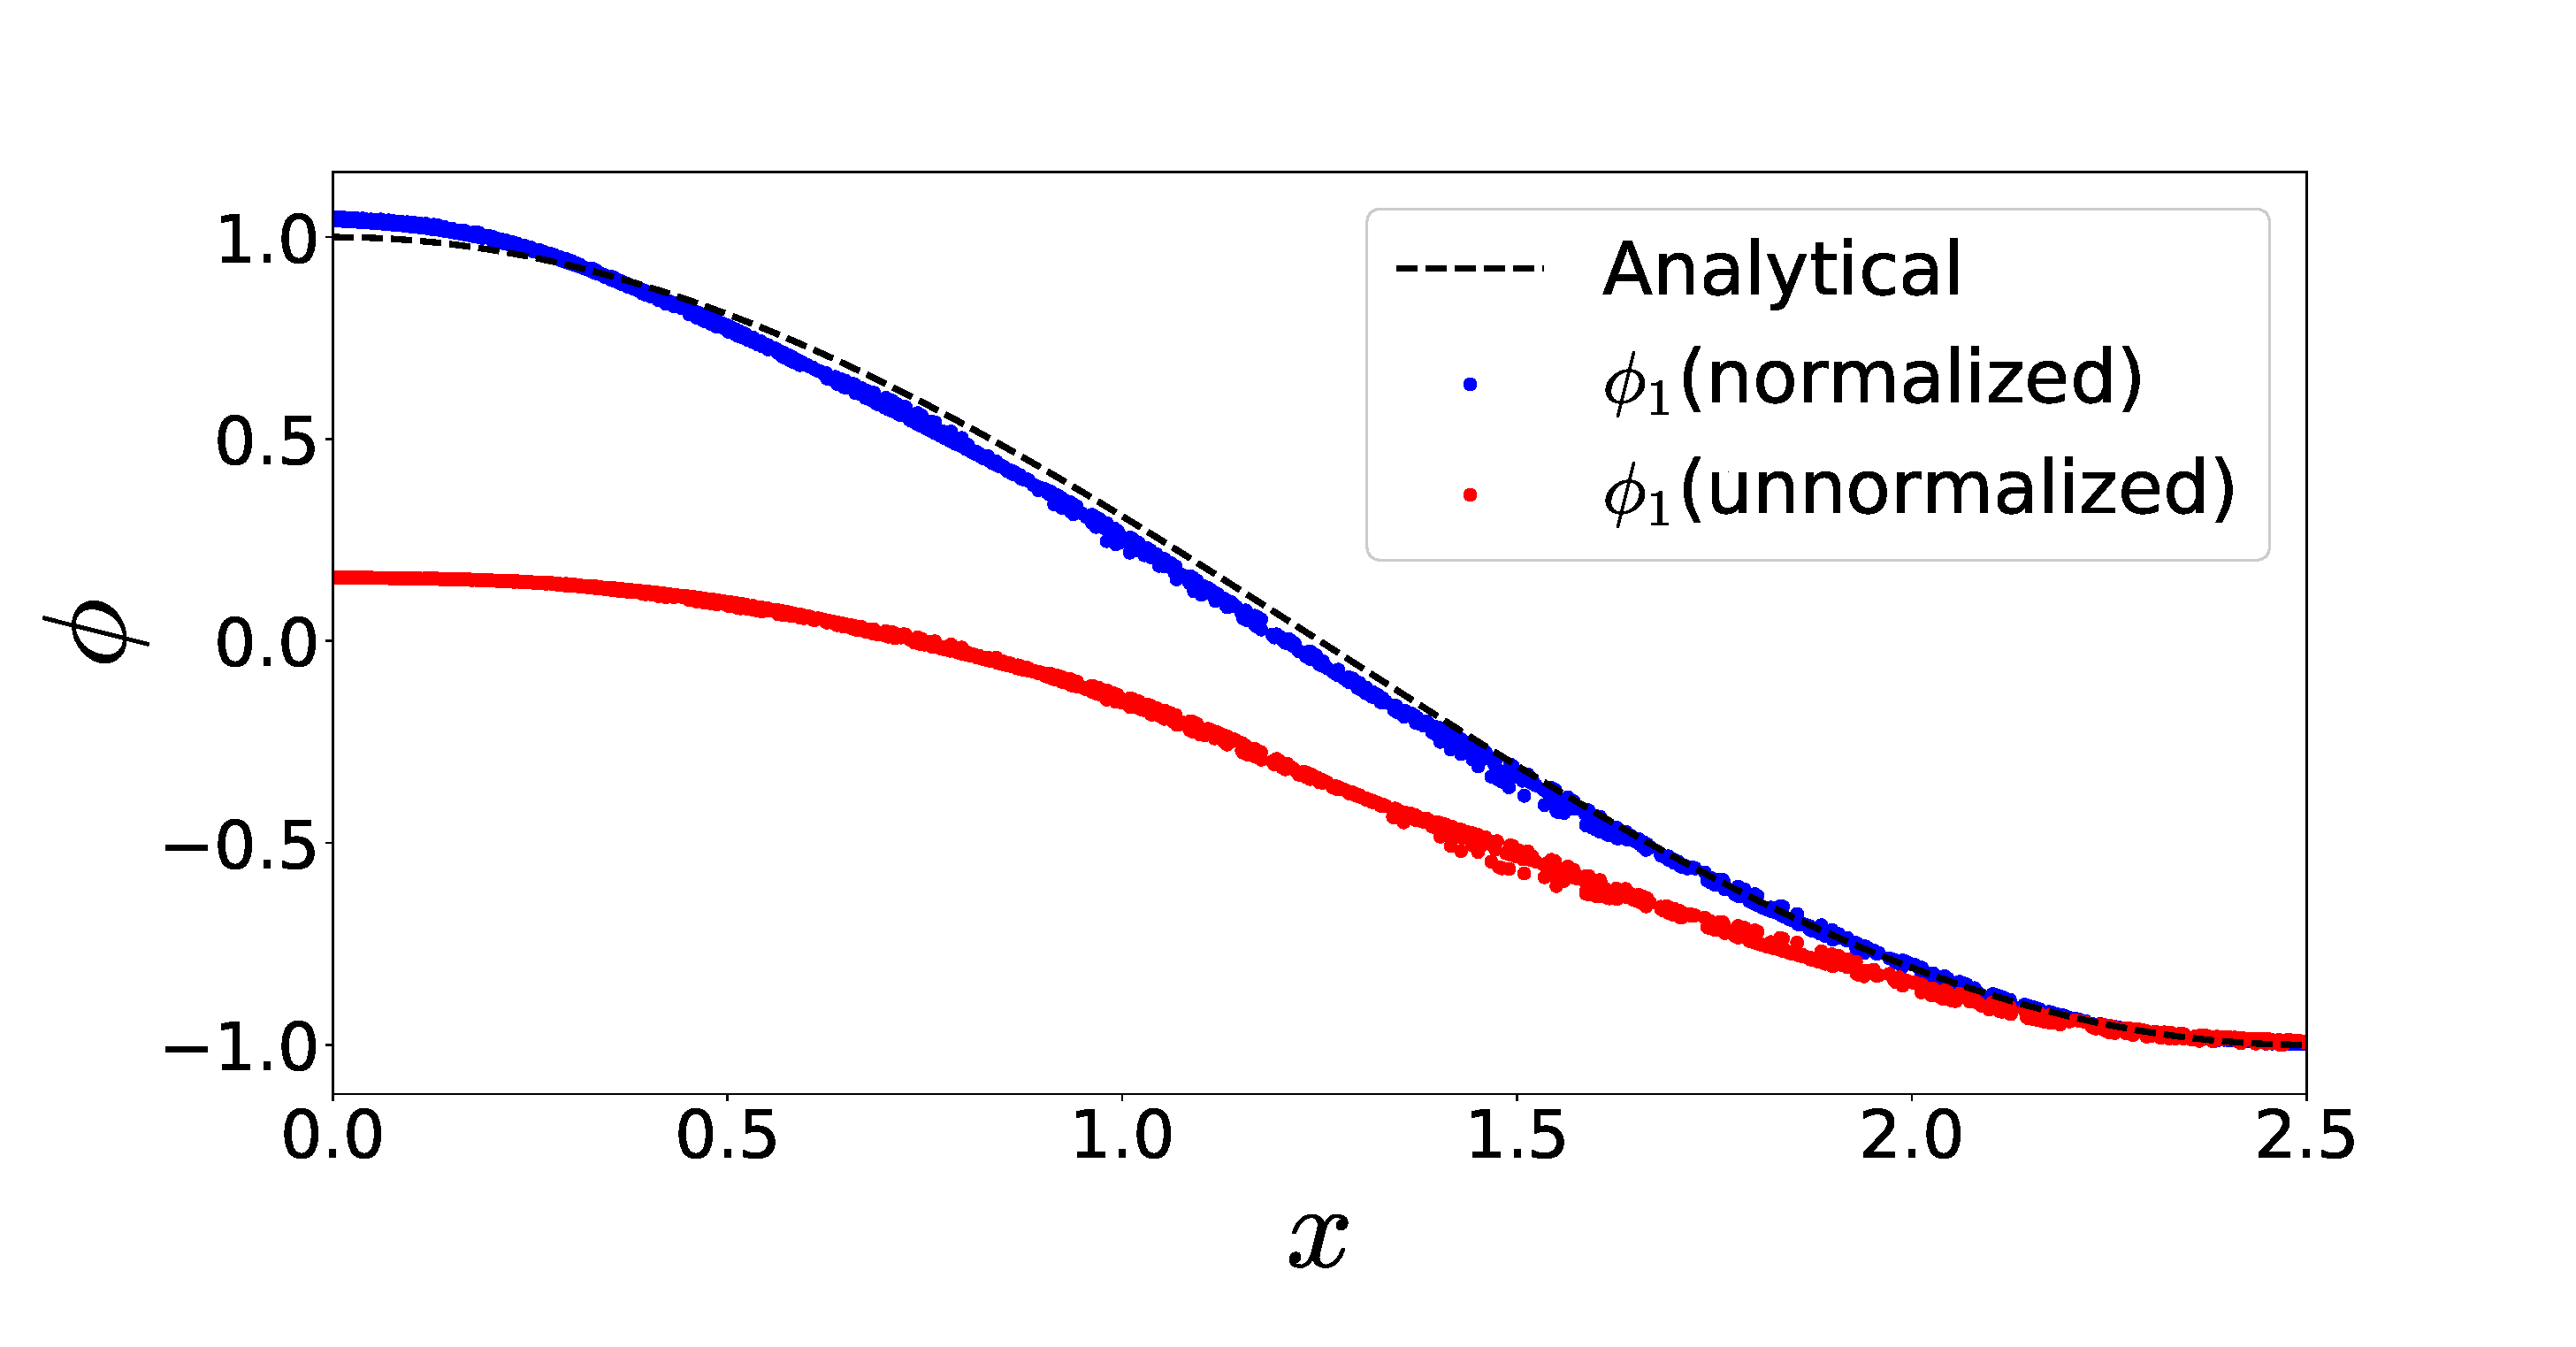
\includegraphics[width=\linewidth]{dmaps-non-x}
    \subcaption{Results for $\phi_1 \approx f_{10}$.}
  \end{subfigure}
  % \hspace{0.5cm}
  \begin{subfigure}[t]{0.45\linewidth}
    \centering
    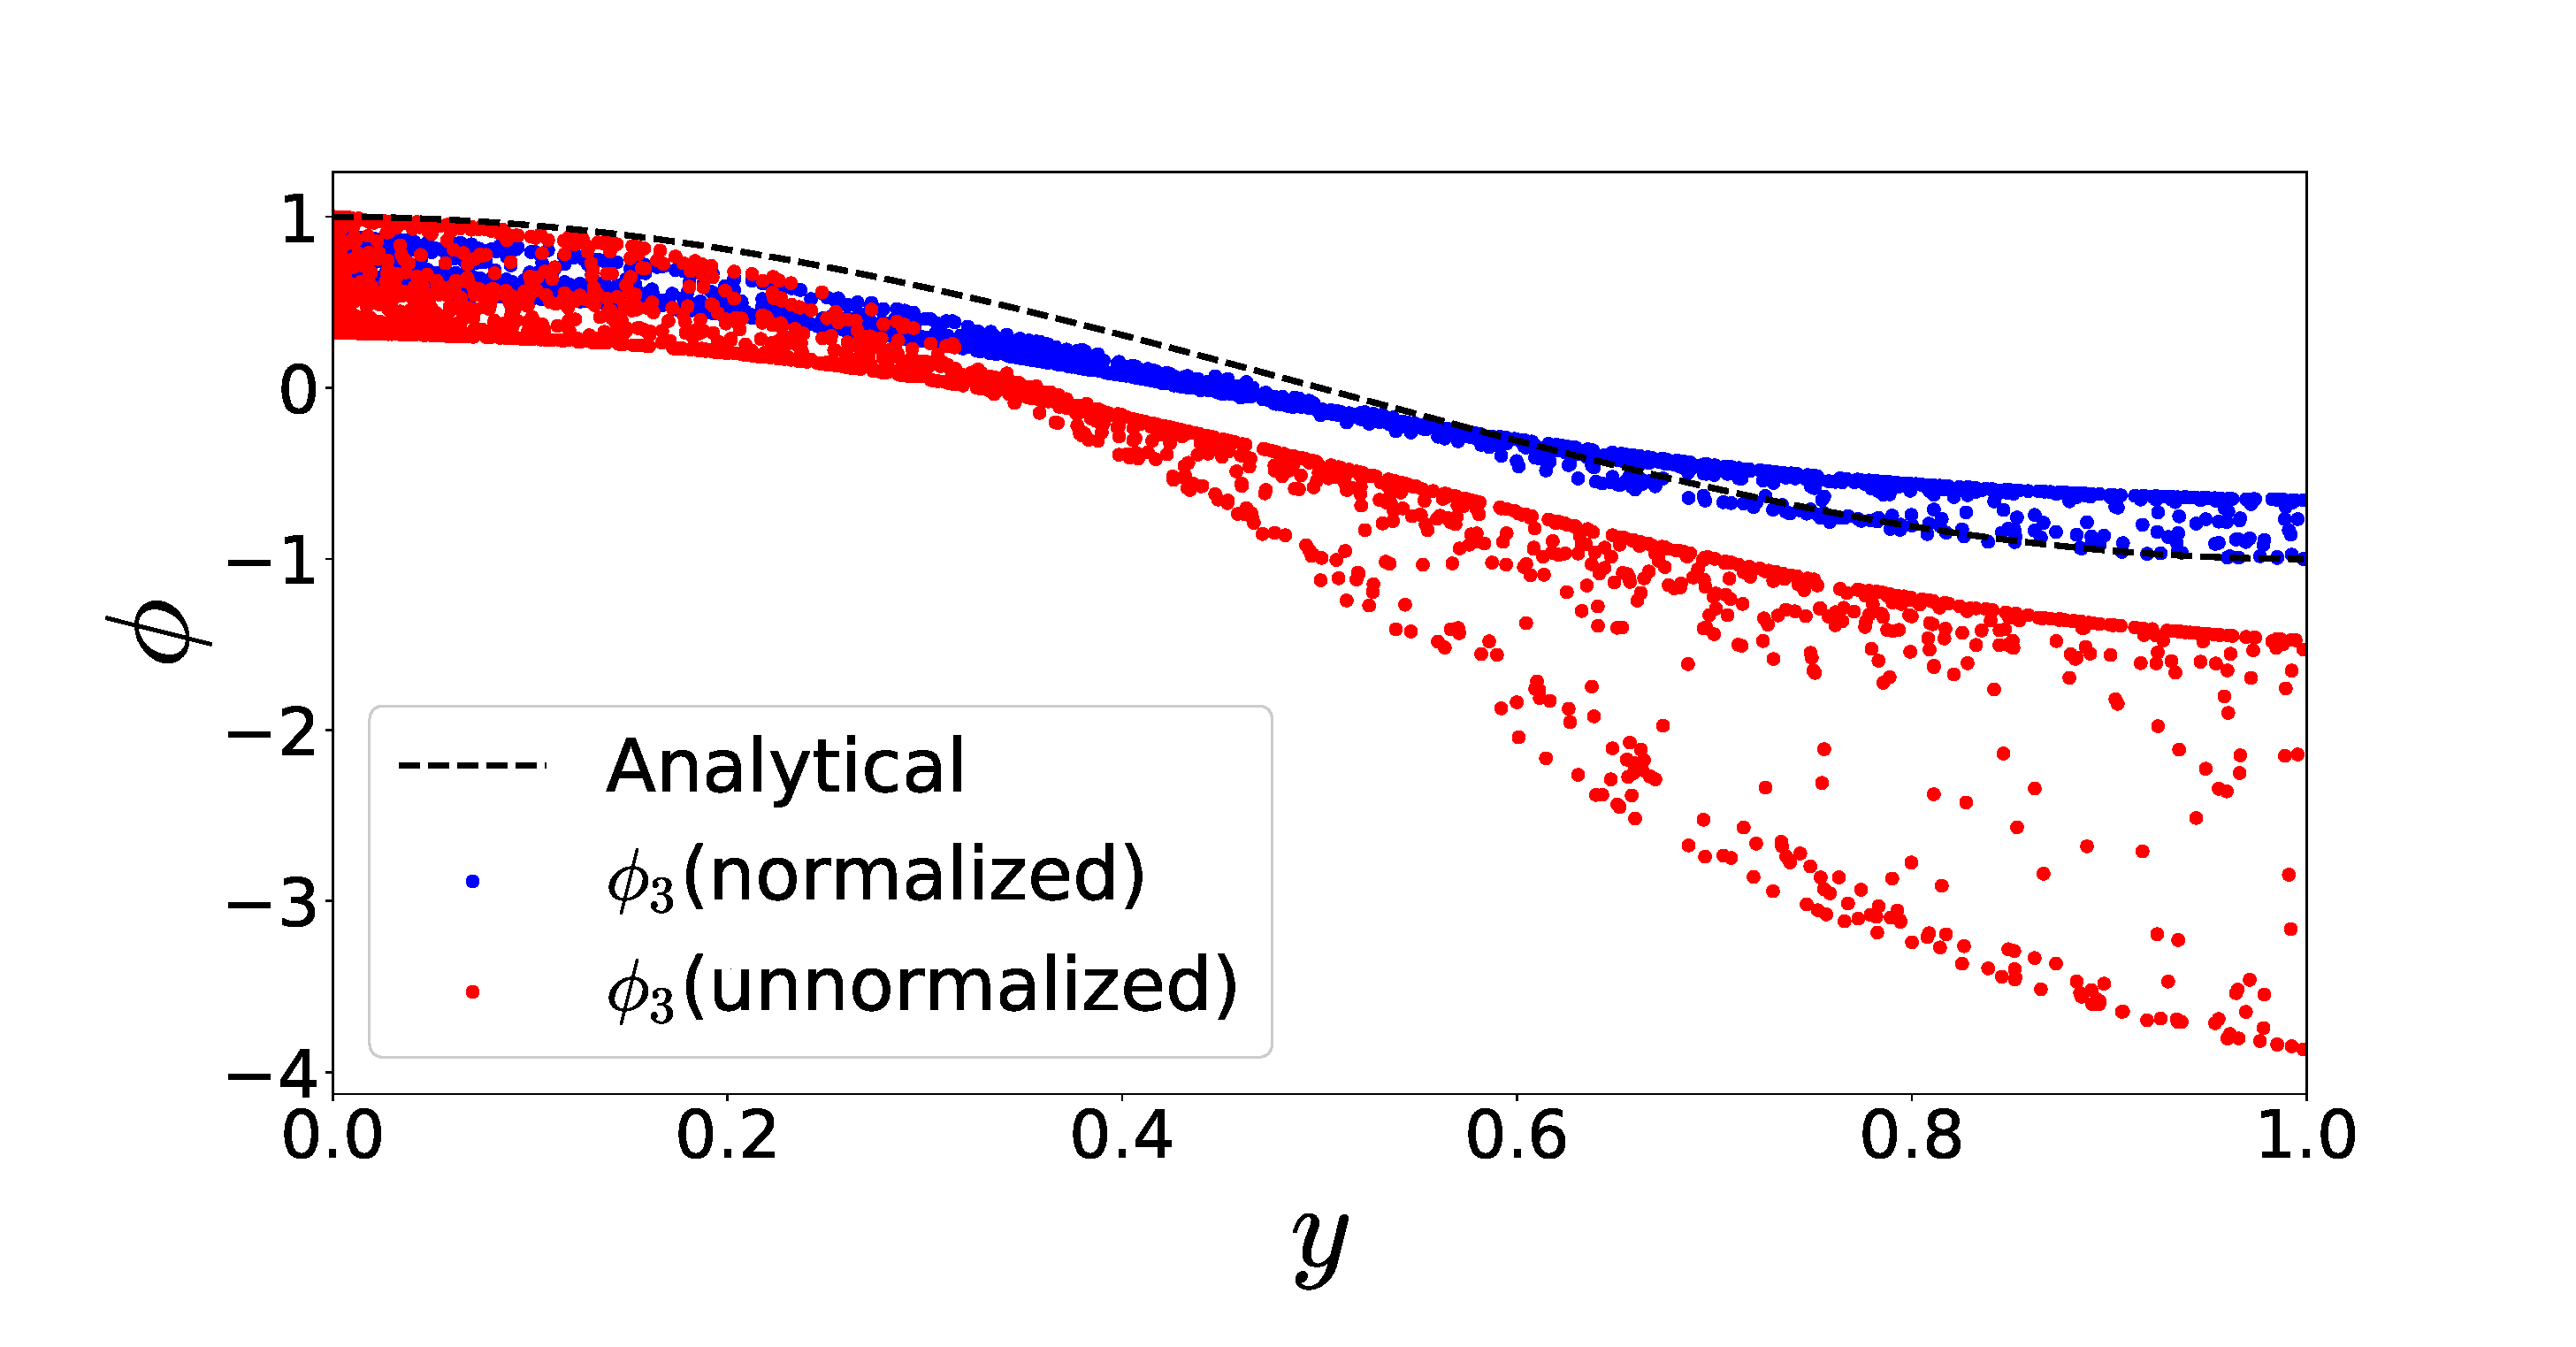
\includegraphics[width=\linewidth]{dmaps-non-y}
    \subcaption{Results for $\phi_3 \approx f_{01}$.}
  \end{subfigure}
  \caption[Comparison of different DMAPS variants]{Comparison of analytical result with normalized and
    unnormalized DMAPS variants showing that the normalized version
    captures the eigenfunctions of the Laplace operator regardless the
    point distribution. \label{fig:dmaps-nonun-phi} }
\end{figure}

The great benefit of DMAPS over PCA is its ability to parameterize
nonlinear manifolds. This comes at the cost of interpretability, as we
now lack an explicit connection between the input, $X$, and the output
$\phi_i$. In certain numerical applications this understanding is
unimportant. When one is interested in an intuitive physical
interpretation of the low-dimensional description, the DMAPS output
can be used to test hypotheses about which variable combinations are
significant.

%%% Local Variables: ***
%%% mode:latex ***
%%% TeX-master: "../../thesis.tex"  ***
%%% End: ***
\section{Equation-free modeling\label{sec:ef}}

The second key component in the work that follows is Equation Free
(EF) modeling. This framework enables one to analyze agent-based
simulations such as social network evolution or molecular dynamics
using systems-level algorithms without deriving explicit, analytical
equations governing the properties of interest
\cite{gear_equation-free_2003,kevrekidis_equation-free:_2004}. EF
modeling has been used to accelerate simulations, to locate coarse
steady states, and to perform bifurcation analysis, using only the
sort of fine-scale simulations that researchers across disciplines
increasingly rely on to model their
problems~\cite{tsoumanis_coarse-graining_2012,ferguson_systematic_2010,bold_equation-free_2014}. We
will now provide an overview of the general framework, and a
particular application known as coarse projective integration.

EF techniques rely on two complementary algorithmic elements: a
restriction operator $\Res$ that maps fine-scale simulations to coarse
variables, and a lifting operator $\Li$ that maps coarse variables to
consistent fine-scale simulations. Thus lifting is the inverse of
restriction, so $\Res \cdot \Li (x) = x$. We will denote the state of
the fine system by $u(t)$, with $U(t)$ the corresponding coarse
state. $u(t)$ could represent the evolving state of neurons in a
simulation of brain activity, while $U(t)$ may track the average
action potential. In such complex models it is difficult to derive an
explicit formula governing the progression of $U(t)$, but by
periodically measuring this quantity as the simulation progresses,
through $\Res: u \rightarrow U$, we can estimate its trajectory. Then,
using an integration scheme as simple as forward Euler, we may
approximate the value of $U(t)$ at some future time,
$U(t + \Delta t)$. Using $\Li: U \rightarrow u$ we obtain a fine-scale
state $u(t + \Delta t)$. This process of alternately restricting and
lifting can be repeated until the system has reached a desired
state. Overall, the result is an accelerated simulation as we have
replaced $\Delta t$ expensive, full-system steps with a single, cheap
application of forward Euler during each iteration. This method is
known as coarse projective integration (CPI), and it is illustrated in
Fig.~\ref{fig:cpi-ill}. This forms the backbone of EF modeling, and in
Chapter~\ref{ch:graphs} we will see how CPI can be used to implement a
stationary-state solver for evolving networks.

\begin{figure}
  \centering
  \includegraphics[width=0.8\textwidth]{cpi-intro}
  \caption[Illustration of coarse projective integration]{Illustration
    of CPI procedure in which repeated applications of the restriction
    operator $\Res$ are used to approximate the trajectory of $U(t)$
    and to estimate its value at some future time $U(t + \Delta
    t)$. Subsequent application of $\Li$ allows one to iterate this
    process, accelerating simulations. \label{fig:cpi-ill}}
\end{figure}

%%% Local Variables: ***
%%% mode:latex ***
%%% TeX-master: "../../thesis.tex"  ***
%%% End: ***


% It is my hope that the
% work presented in this thesis will be viewed as a small advance in
% this larger march. 

% % % % possible first sentences of thesis

% The following chapters are a test of the theory that engineering
% theses are never read, neither by their advisor nor original
% author. Instead, the theory asserts that the author vomits the
% document into existence in a violent storm of anxiety and
% anticipation, never to be perused again.

% There are those that do brave battle with the big data and there are
% those that survey the wasted battlefield, strewn with broken
% algorithms and bad statistics, and run towards the siren sound of
% Excel. But there is no escape. Some of the warrior's
% deeds were recorded so that future generations would know the folly of
% csv files; the following documents were recovered from the battlefield
% of nonlinearities. Let them be a lesson to all.

% It is not uncommon for the modern researcher to pore over his
% gigabytes of data and question what it is all for.

% Should your data remain big for over six hours after reading this
% thesis, please consult your nearest graduate student.

% Modern researchers are often confronted by the unnecessarry bigness
% of their datasets and wish to make them smaller. This can occur for a
% variety of reasons. 

% Despite growing demand for algorithms that work good, scientists
% are unable to make them good.

% It is no secret that big data requires big algorithms.

%%% Local Variables: ***
%%% mode:latex ***
%%% TeX-master: "../../thesis.tex"  ***
%%% End: ***